\documentclass[a4paper]{article}
\usepackage{polski}
\usepackage[utf8]{inputenc}
\usepackage{amsmath}
\usepackage{graphicx}
\usepackage{caption}
\usepackage{subcaption}
\usepackage{geometry}
\usepackage{float}

\newcommand{\matr}[1]{\mathbf{#1}} % undergraduate algebra version

\graphicspath{{./img/}}

\title{MGR - Raport 1}
\author{Jakub Postępski}

\begin{document}

\maketitle

\section{Problem}
Należy skompensować siłę grawitacji w układzie ze sprężyną. Rozwiązaniem jest określenie masy a następnie dodanie odpowiednich sił do układu w celu kompensacji siły grawitacji.

\section{Obiekt}
Obiektem jest układ ze sprężyną i amortyzatorem. Na końcu zawieszona jest punktowa masa $m$ której grawitację należy skompensować. Przyjmujemy że dla użytkownika dostępne są pomiary położenia ($x$), prędkości ($\dot{x}$), przyspieszenia ($\ddot{x}$) oraz siły odczytanej przez czujnik.

Model obiektu można opisać układem równań różniczkowych:

\begin{equation}
	\begin{bmatrix}
	    \dot{x} \\
	    \ddot{x}
	\end{bmatrix}
	=
	\begin{bmatrix}
	    0 & 1 \\
	    \frac{k}{m} & \frac{b}{m}
	\end{bmatrix}
	\begin{bmatrix}
		x \\
	    \dot{x}
	\end{bmatrix}
	+
	\begin{bmatrix}
	    0 \\
	    1
	\end{bmatrix}
	{-g + u_w}
\end{equation}

gdzie:
\begin{itemize}
	\item $x$ pozycja zawieszonej masy
	\item $k$ parametr sztywności
	\item $b$ parametr amortyzacji
	\item $m$ masa przedmiotu
	\item $g$ przyspieszenie ziemskie
	\item $u_w$ przyspieszenie które można zewnętrznie dodać do układu
\end{itemize}

Układ możemy więc zapisać w standardowej postaci
\begin{equation}
\dot{x} = \textbf{A}x + \textbf{B}u(t)
\end{equation}
gdzie:
\begin{equation}
\mathbf{A} = 	\begin{bmatrix}
	    0 & 1 \\
	    \frac{k}{m} & \frac{b}{m}
	\end{bmatrix}
\end{equation}
oraz:
\begin{equation}
\mathbf{B} = \begin{bmatrix}
	    0 \\
	    1
	\end{bmatrix}
\end{equation}

Po zdyskretyzowaniu z okresem próbkowania $t$ otrzymujemy układ:
\begin{equation}
x(k+1) = \mathbf{A_d}x(k) + \mathbf{B}_du(k)
\label{eq:dyskretny}
\end{equation}


Symulację obiektu (rys. \ref{fig:system}) można wykonać korzystając z wersji dyskretnej układu. Czujnik siły można zasymulować biorąc przyspieszenie układu $\ddot{x}$ i mnożąć przez masę. W celu symulacji zakłóceń w każdym kroku symulacji zmiennych stanu układu dodawany jest szum biały.

\begin{figure}[H]
	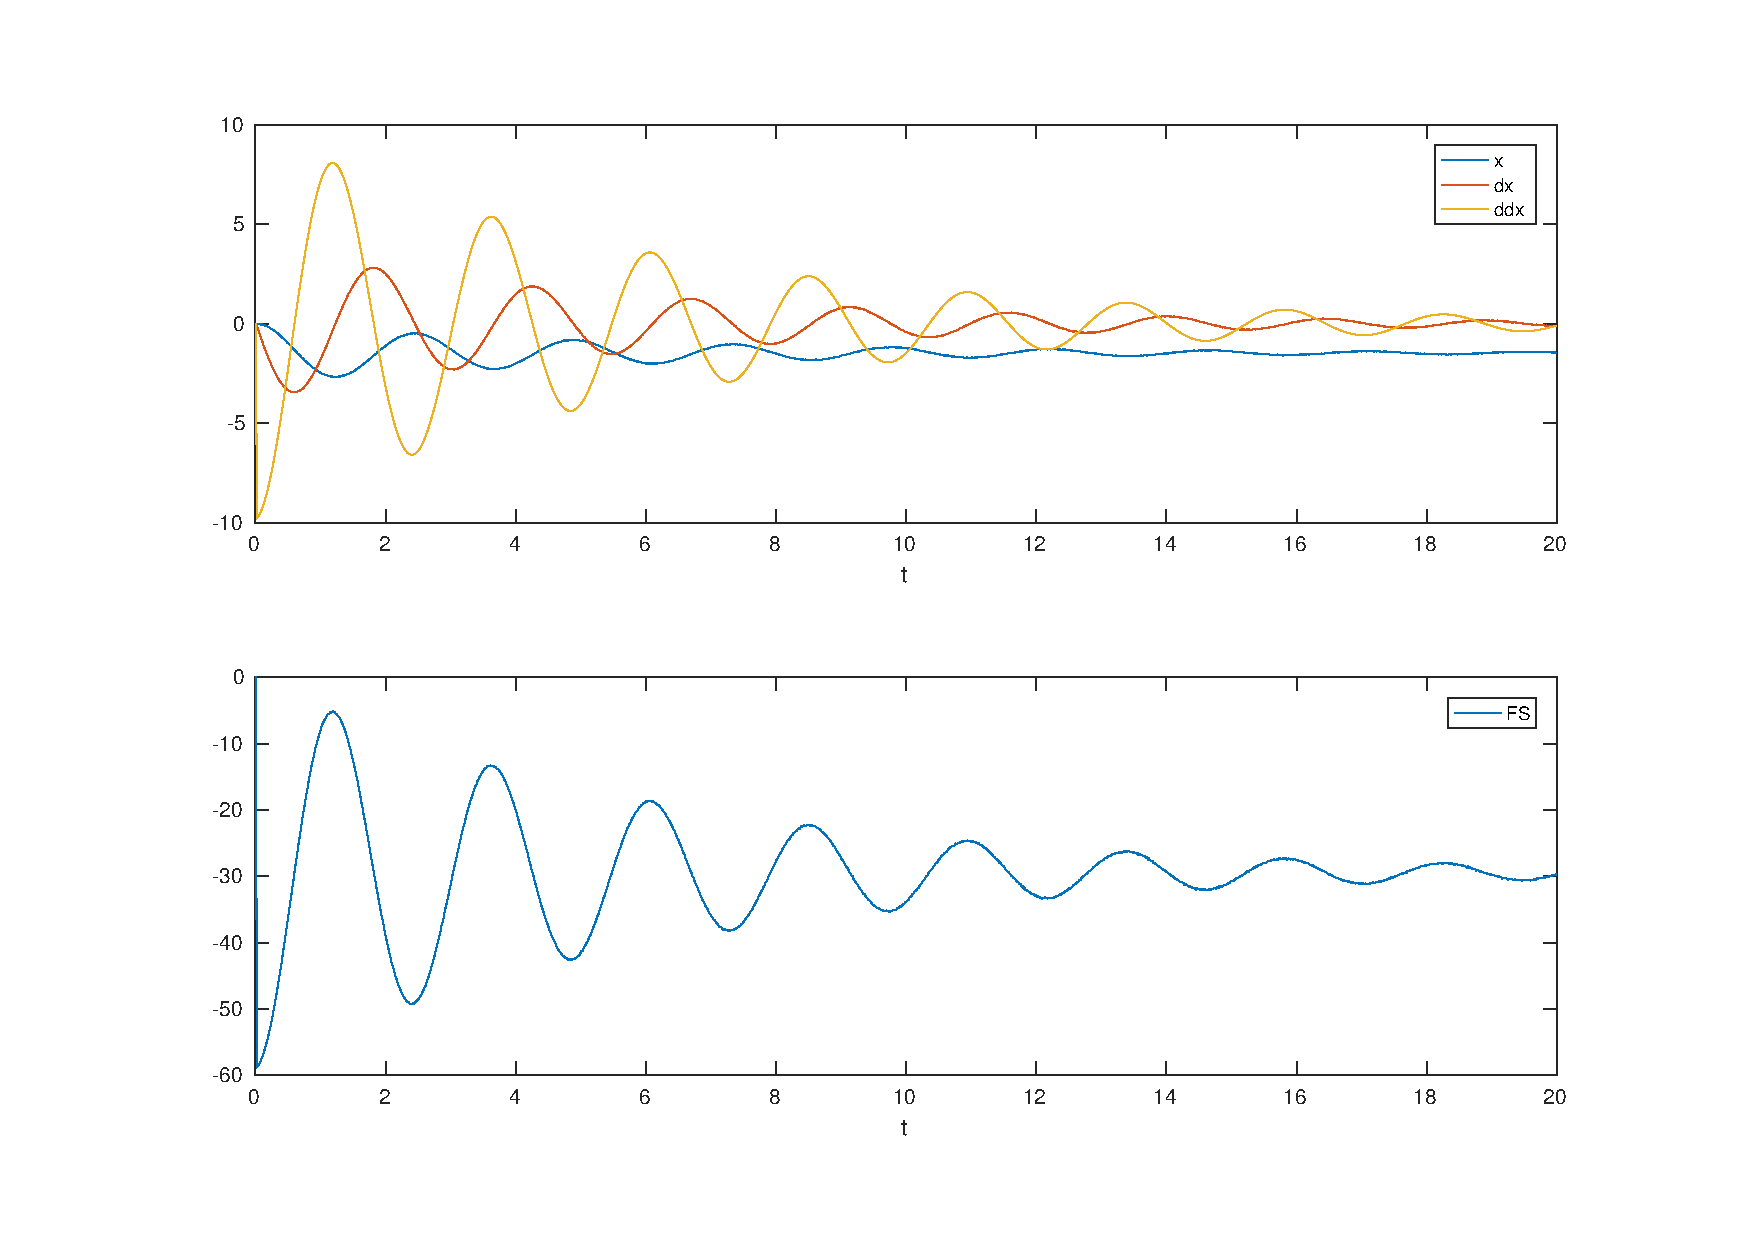
\includegraphics[width=0.99\linewidth]{system_sys}
	\centering
	\caption{Symulacja układu z parametrami $T=0.01$, $k = 20$, $b = 1$, $m = 3$.}
	\label{fig:system}
\end{figure}

\section{Estymacja masy}
Estymacja masy działa na podstawie dwóch modeli. Model opisany w sekcji \ref{fs} działa dobrze gdy układ jest ustabilizowany. Model opisany w sekcji \ref{pos} działa dobrze gdy układ jest w ruchu. W celu poprawnej estymacji w dowolnym momencie pracy układu połączono dane z modeli przy wykorzystaniu logiki rozmytej (rys. \ref{fig:system_mass}). Funkcja przynależności (rys. \ref{fig:system_w}) decyduje o większym udziale modelu czujnika siły w momencie gdy na układ nie działają przyspieszenia.

\begin{figure}[H]
	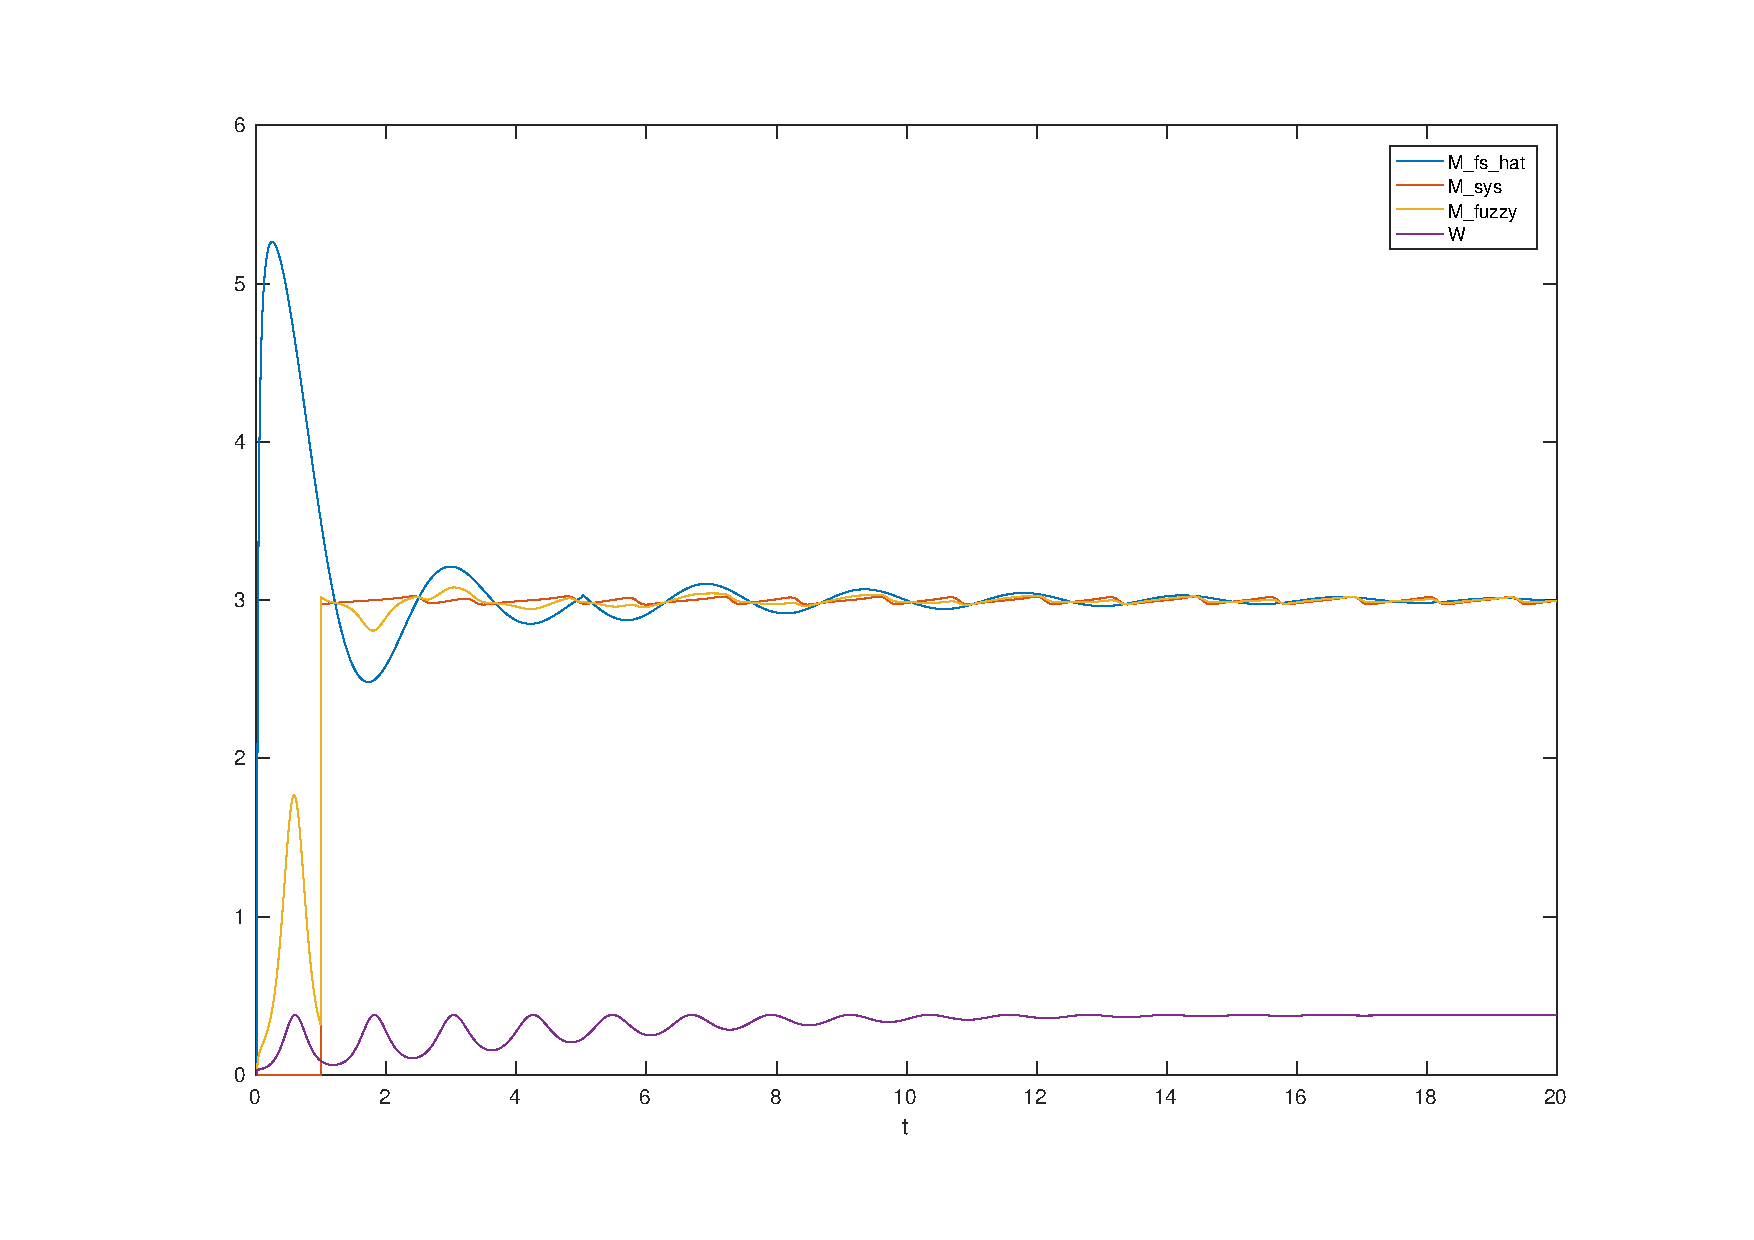
\includegraphics[width=0.99\linewidth]{system_mass}
	\centering
	\caption{Estymacja masy układu z parametrami $T=0.01$, $k = 20$, $b = 1$, $m = 3$. Linią $W$ oznaczono poziom funkcji przynależności modelu }
	\label{fig:system_mass}
\end{figure}

\begin{figure}[H]
	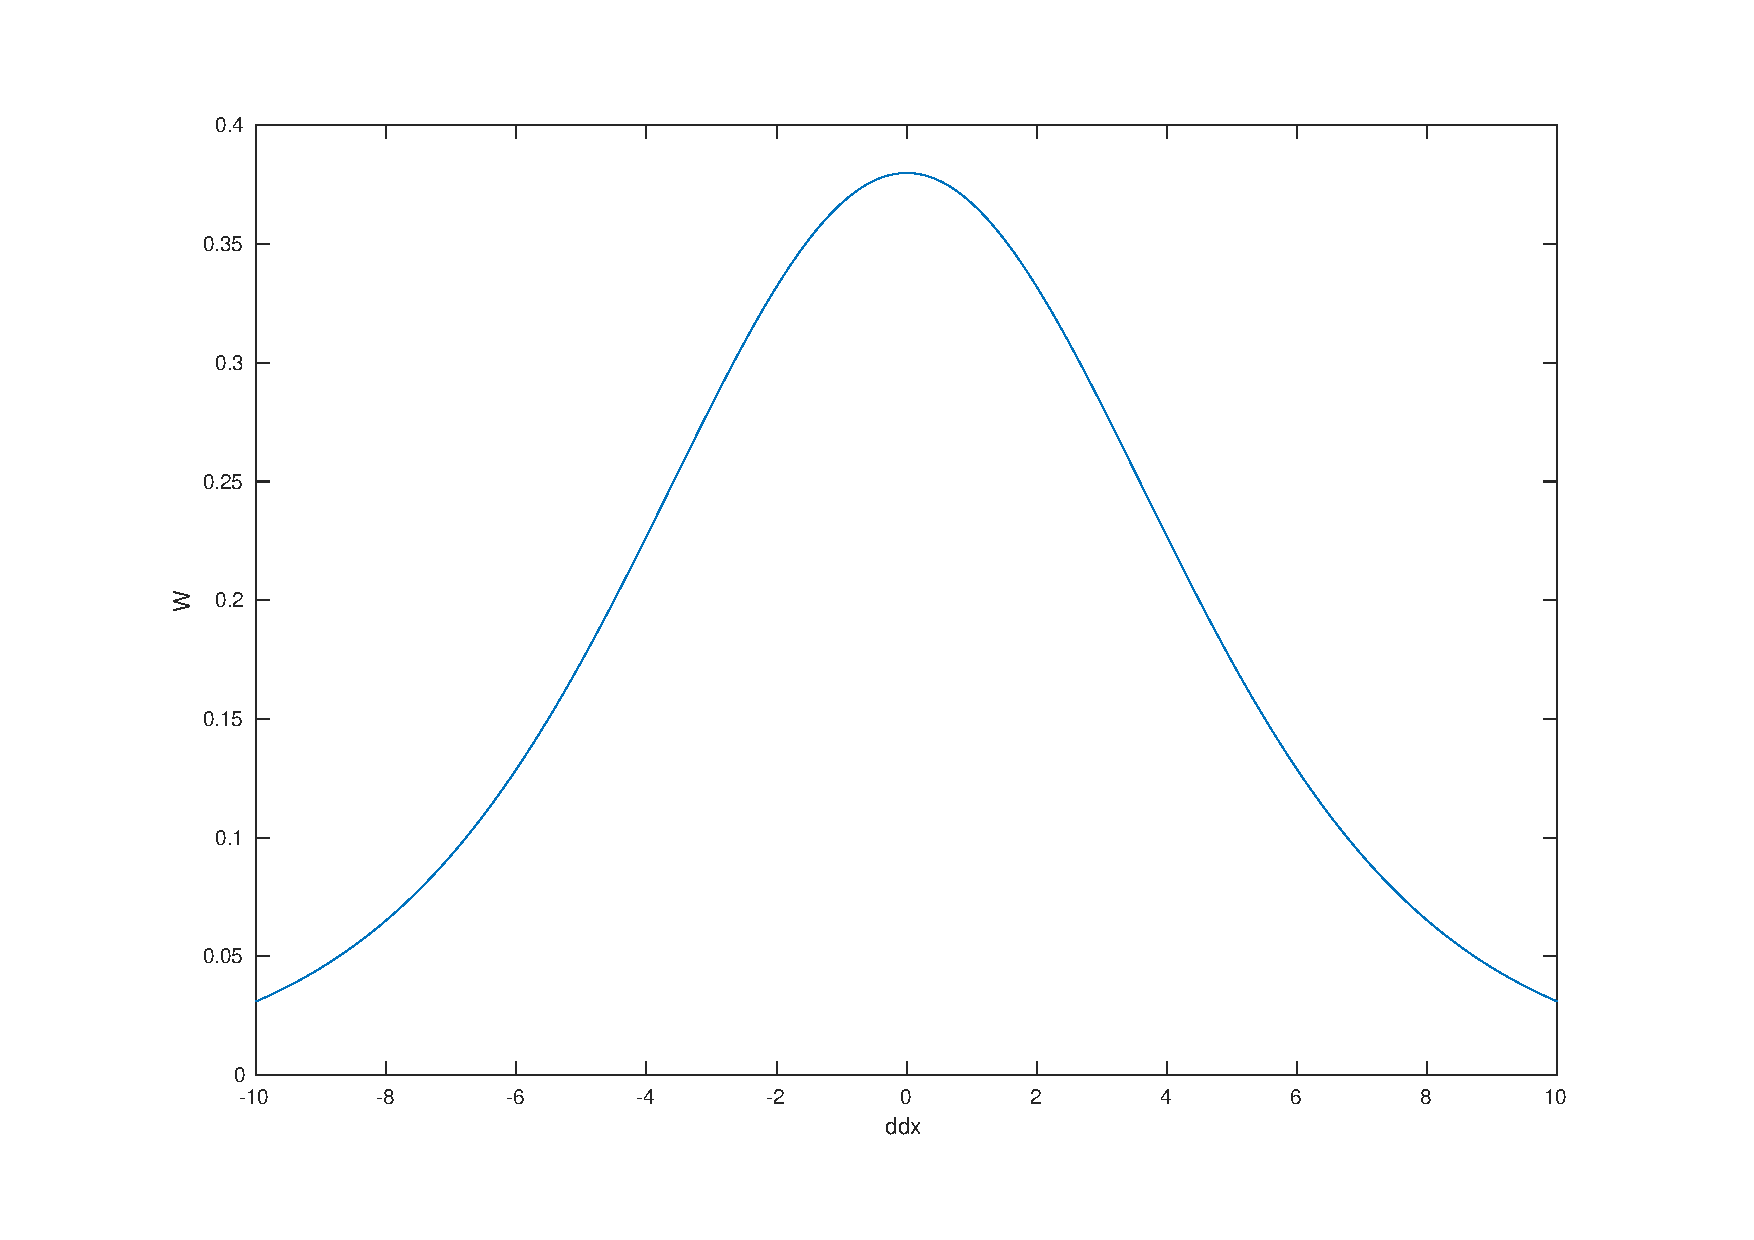
\includegraphics[width=0.99\linewidth]{system_w}
	\centering
	\caption{Sigmoidalna funkcja przynależności postaci $f(\ddot{x}; a, c) = \frac{1}{1+e^{\|\ddot{x}\|-c}}$ z parametrami $a~=~0.4$, $c = 2$.}
	\label{fig:system_w}
\end{figure}



\subsection{Estymacja z czujnika siły}
\label{fs}
Siła odczytywana z czujnika siły jest sumą sił działających na masę. Kiedy masa się nie porusza w łatwy sposób można odczytać siłę grawitacji. W momencie ruchu układu z czujnika dostajemy sygnał zmienny. W celu uzyskania interesującej nas składowej stałej (siła grawitacji) możemy zastosować transformatę Fouriera. Jedną z własności tej transformaty jest fakt że uzyskana składowa stała jest średnią arytmetyczną sygnału. W praktyce w celu uzyskania siły grawitacji stosowana jest średnia krocząca która działa podobnie do filtru dolnoprzepustowego. Dodatkową zaletą zastosowania filtru odfiltrowywanie szumów pomiarowych.

W trakcie symulacji eksperymentalnie dobierano ilość próbek branych pod uwagę przez filtr. Dla filtrów z krótkim oknem (rys. \ref{fig:systemfs4_mass}, \ref{fig:systemfs100_mass}) widać, że są w stanie odfiltrować jedynie szumy pomiarowe czujnika. Dla filtrów z długim oknem widać, że potrzeba dużo czasu aby otrzymać estymację masy (rys. \ref{fig:systemfs1000_mass}). Finalnie wybrano okno długości $n = 500$ (rys. \ref{fig:systemfs500_mass}.)

\begin{figure}[H]
	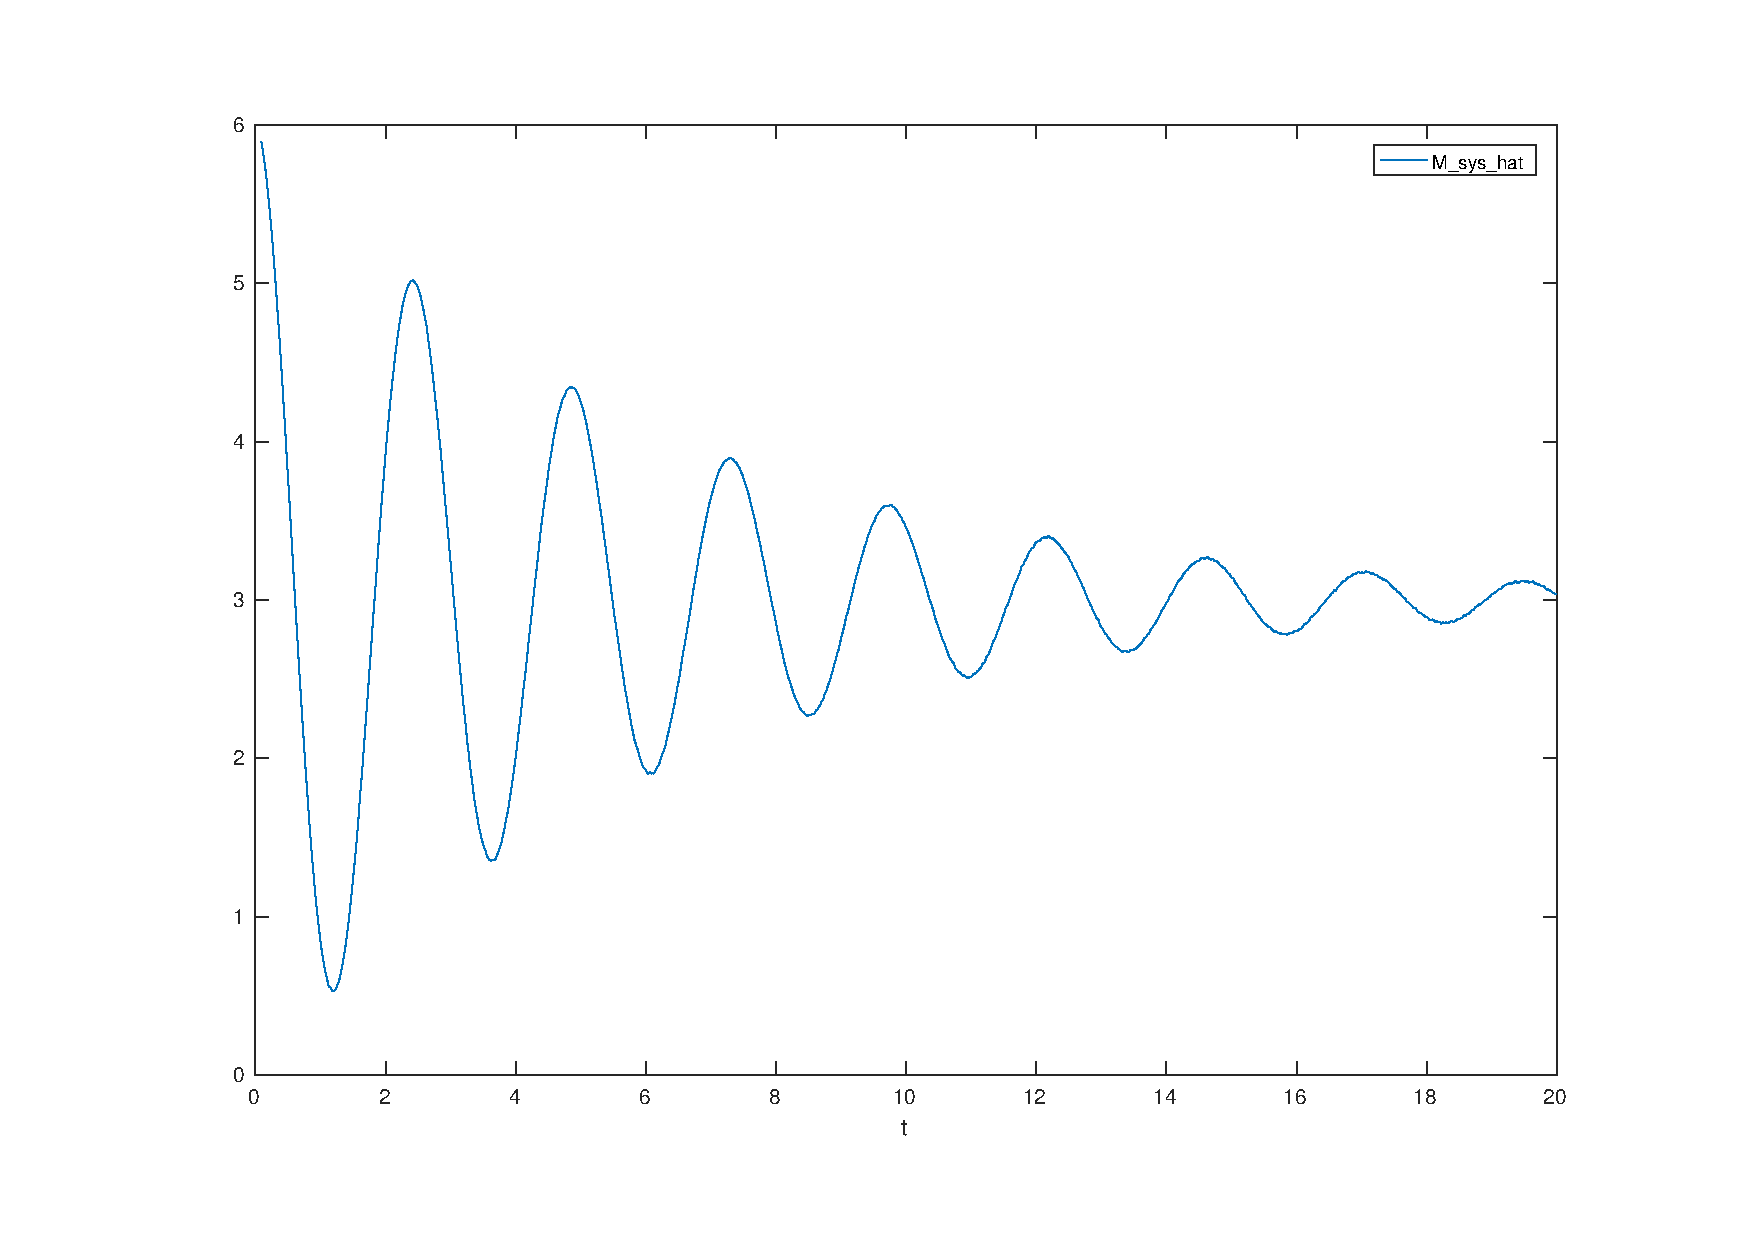
\includegraphics[width=0.99\linewidth]{systemfs4_mass}
	\centering
	\caption{Estymacja masy układu z parametrami $T=0.01$, $k = 20$, $b = 1$, $m = 3$ dla 4 próbek używanych w alogrytmie średniej kroczącej. }
	\label{fig:systemfs4_mass}
\end{figure}

\begin{figure}[H]
	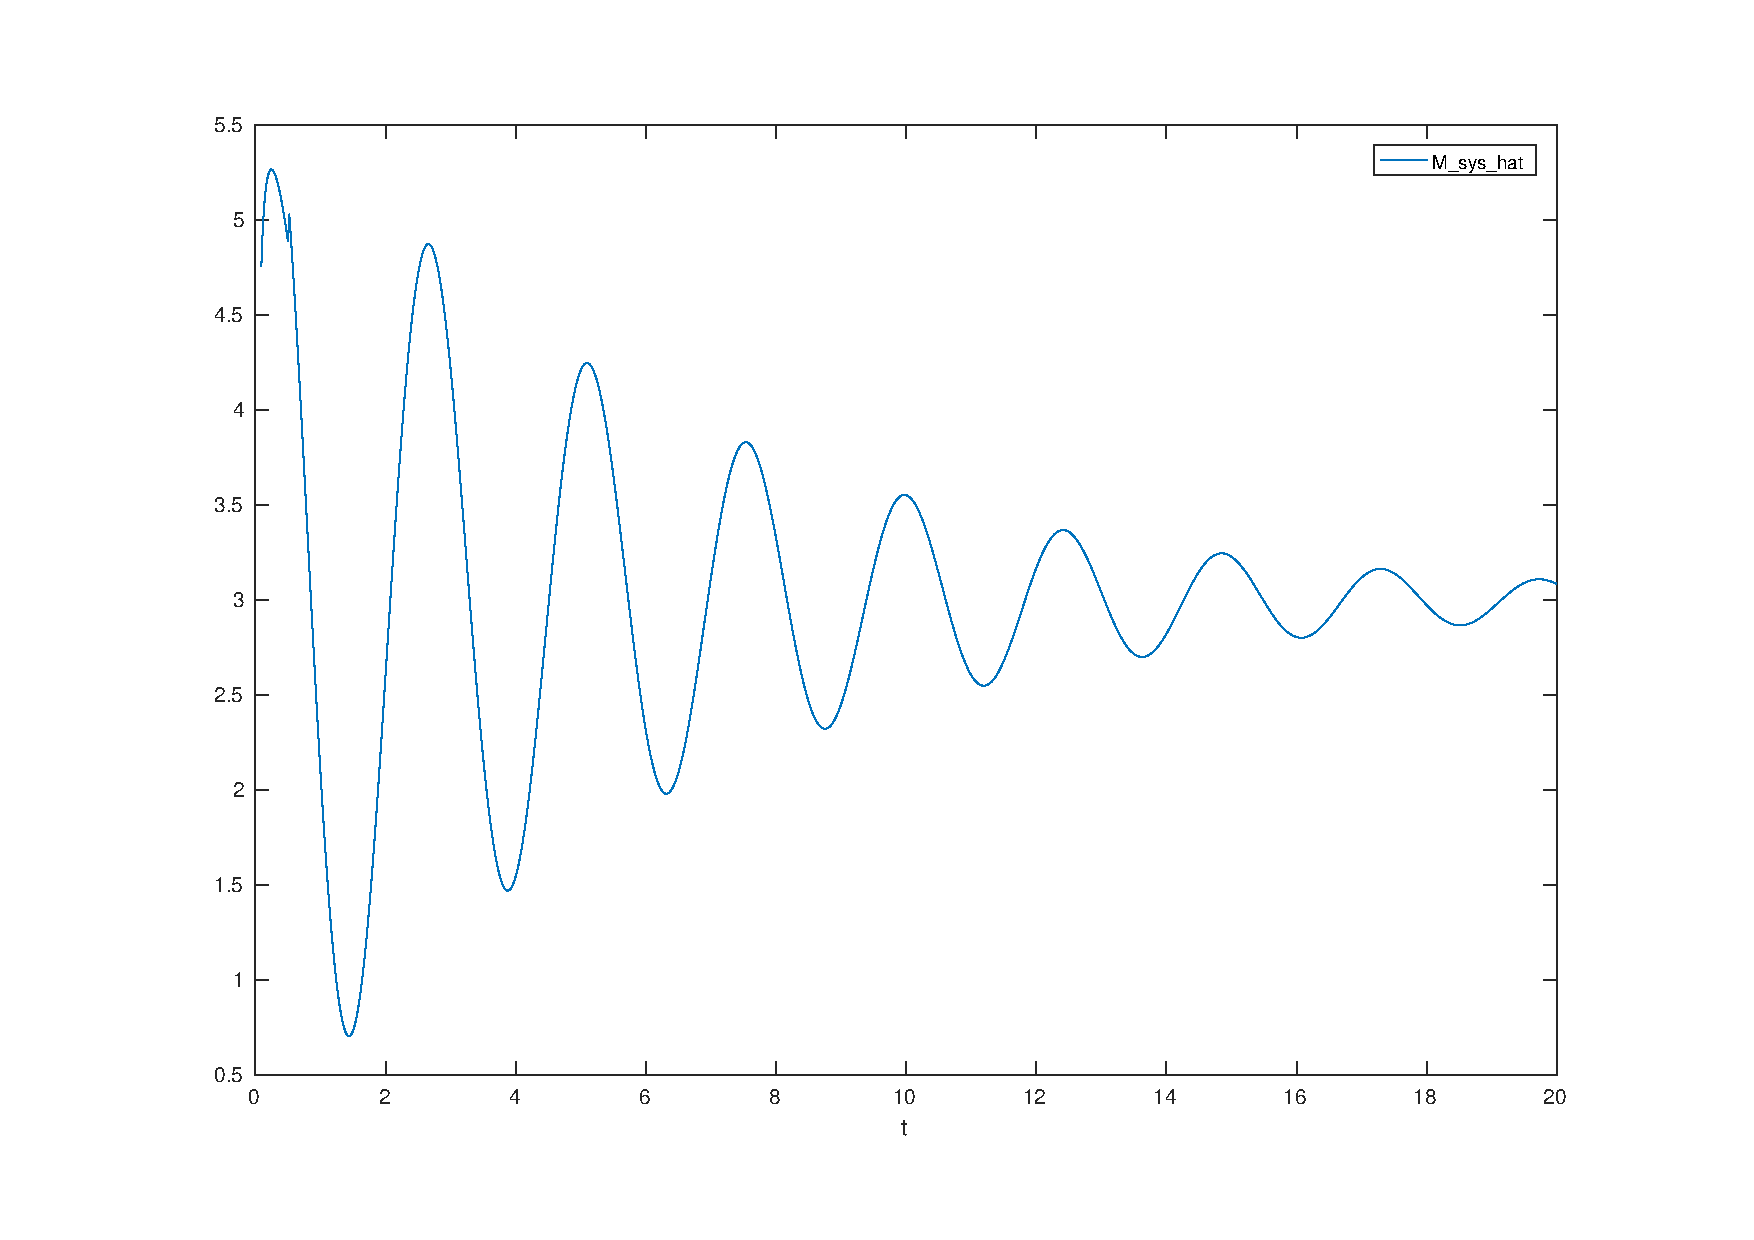
\includegraphics[width=0.99\linewidth]{systemfs100_mass}
	\centering
	\caption{Estymacja masy układu z parametrami $T=0.01$, $k = 20$, $b = 1$, $m = 3$ dla 100 próbek używanych w alogrytmie średniej kroczącej.}
	\label{fig:systemfs100_mass}
\end{figure}

\begin{figure}[H]
	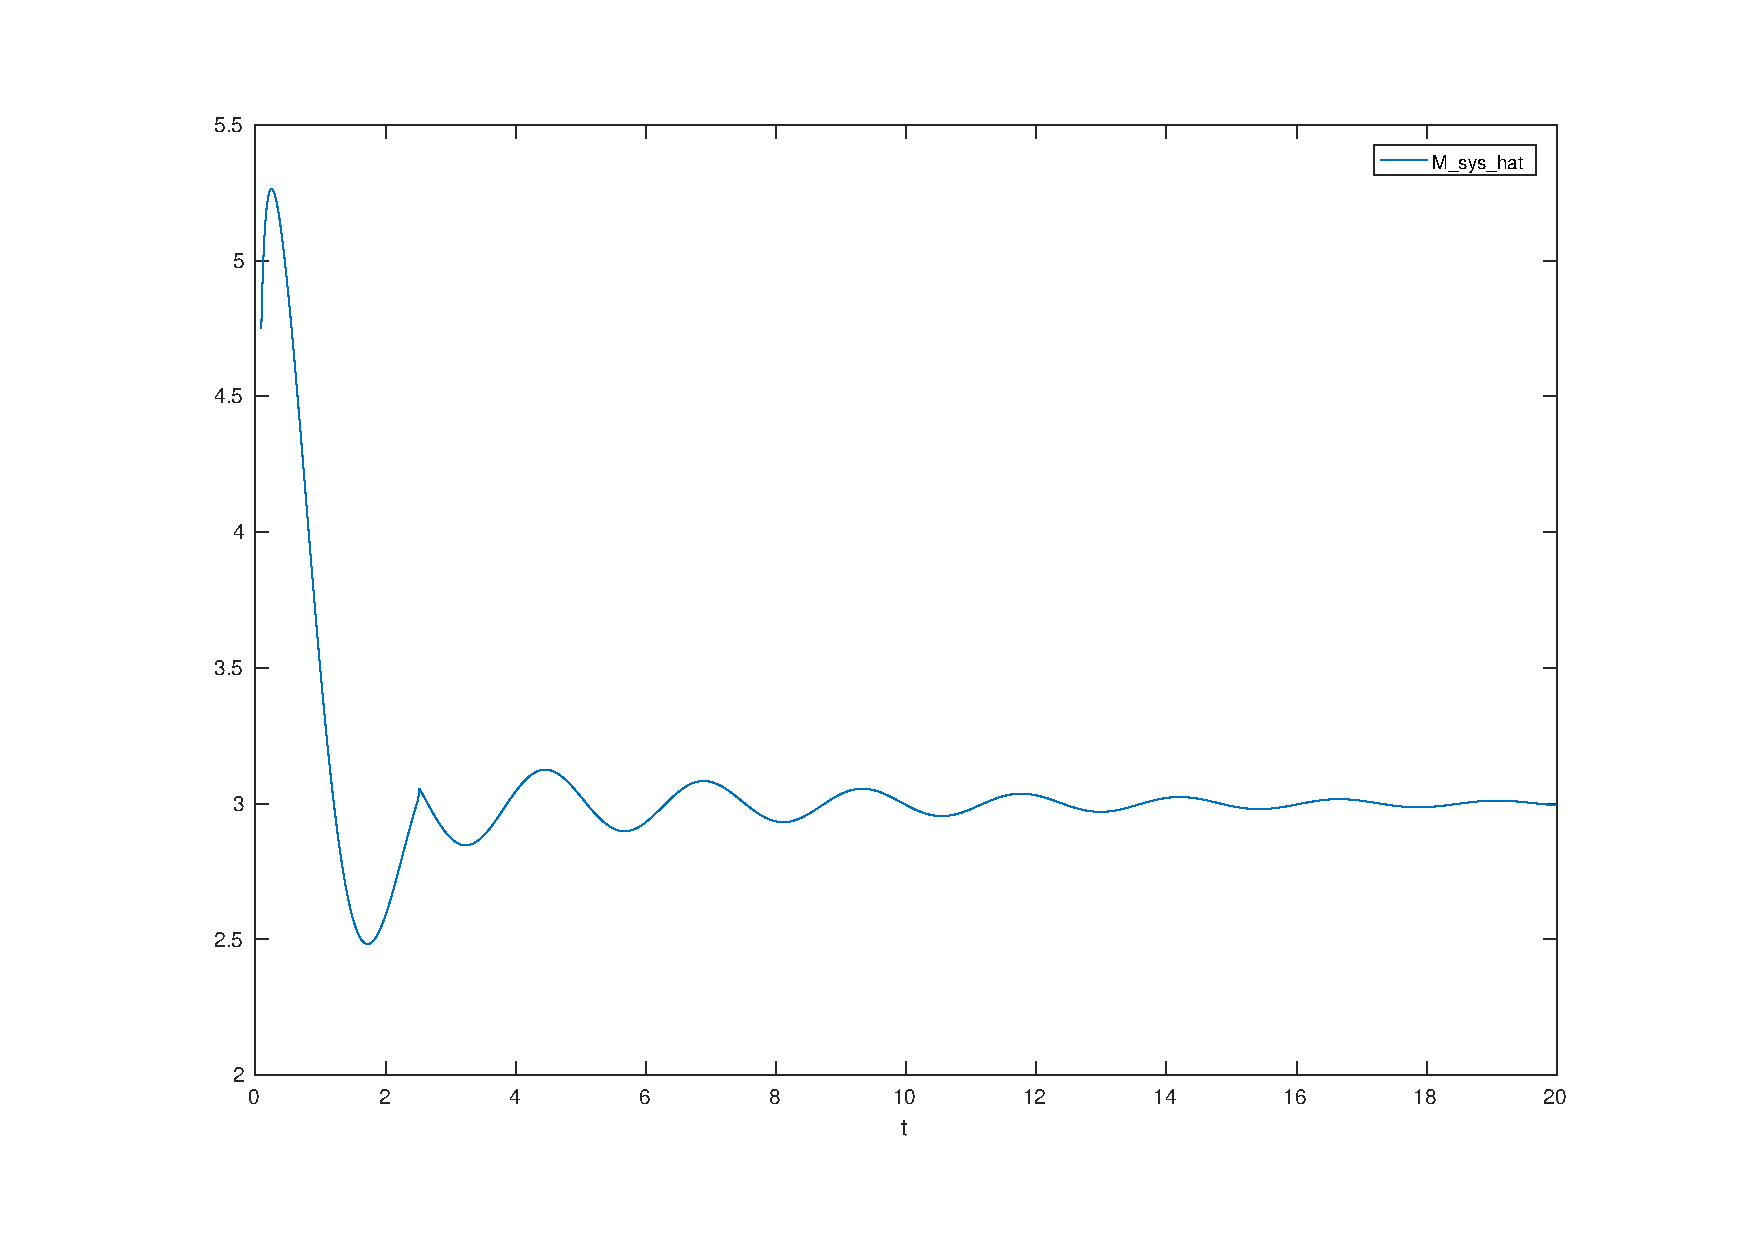
\includegraphics[width=0.99\linewidth]{systemfs500_mass}
	\centering
	\caption{Estymacja masy układu z parametrami $T=0.01$, $k = 20$, $b = 1$, $m = 3$ dla 500 próbek używanych w alogrytmie średniej kroczącej.}
	\label{fig:systemfs500_mass}
\end{figure}


\begin{figure}[H]
	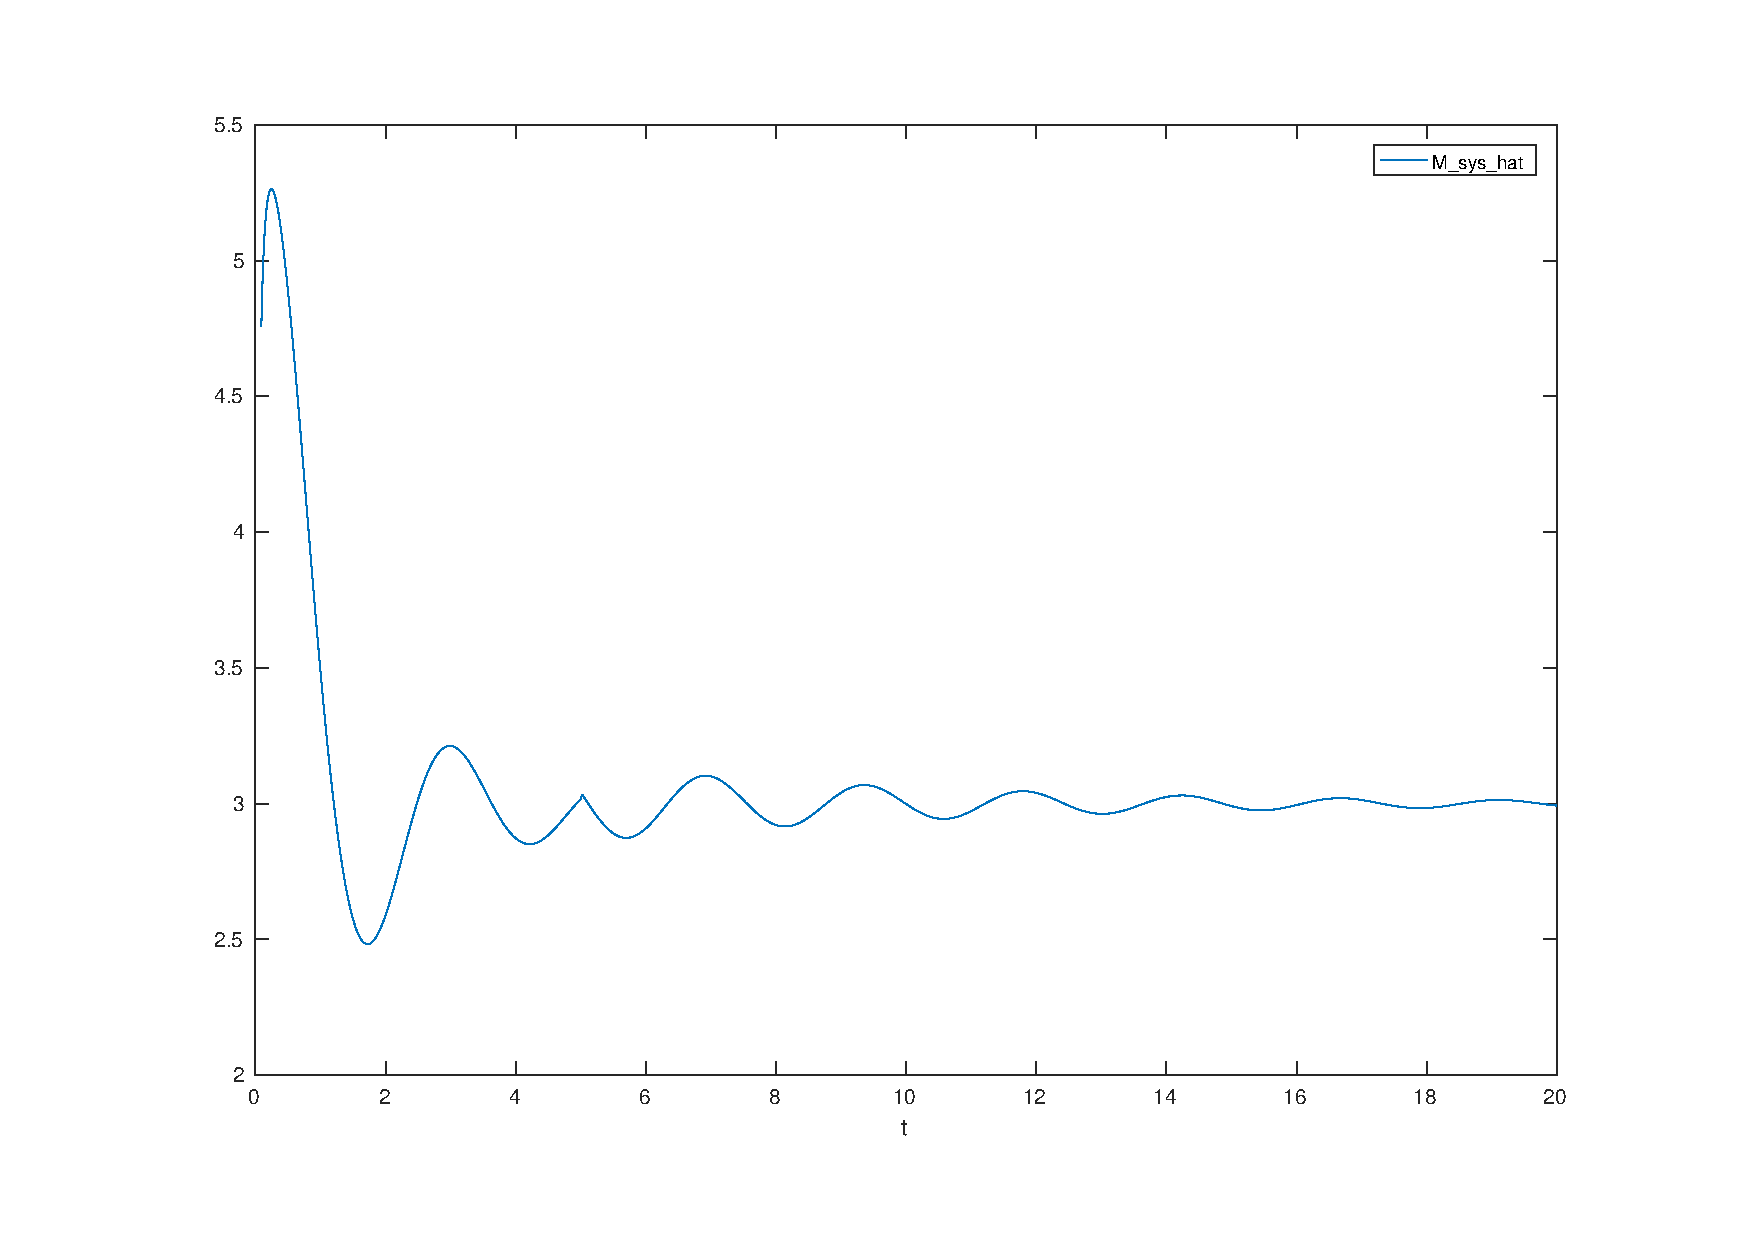
\includegraphics[width=0.99\linewidth]{systemfs1000_mass}
	\centering
	\caption{Estymacja masy układu z parametrami $T=0.01$, $k = 20$, $b = 1$, $m = 3$ dla 1000 próbek używanych w alogrytmie średniej kroczącej. }
	\label{fig:systemfs1000_mass}
\end{figure}


\subsection{Estymacja z macierzy układu}
\label{pos}
Ponieważ macierz $\mathbf{B}$ ma tylko jeden wyraz różny od zera $\mathbf{B_d}$ jest uzyskiwana w prosty sposób i można przyjąć że:
\begin{equation}
\mathbf{B_d} = \mathbf{B}T
\end{equation}
Przekształcając równanie \ref{eq:dyskretny} i stosując pseudoinwersję macierzy otrzymujemy równanie macierzowe:
\begin{equation}
	\mathbf{A_d} = (X(k+1) - \mathbf{B}_du(k))(X(k))^{pinv}
	\label{eq:pinv}
\end{equation}
przy założeniu $n$ ostatnich próbek zmiennych stanów układu
\begin{equation}
	X(k) = 	\begin{bmatrix}
		    x(k) & x(k-1)  & ... & x(k-n)
		\end{bmatrix}
	\label{eq:xk}
\end{equation}

Po obliczeniu estymacji $\mathbf{A_d}$ metodą ZOH wyliczamy estymację macierzy $\mathbf{A}$ otrzymując macierz
\begin{equation}
\mathbf{\hat{A}} = 	\begin{bmatrix}
	    a_{11} & a_{12}\\
	    a_{21} & a_{22}
	\end{bmatrix}
\end{equation}
Po przyrównaniu jej do macierzy $\mathbf{A}$ możemy wyliczć masę z równań:
\begin{equation}
\hat{m_1} = \frac{-k}{a_{21}}
\end{equation}
\begin{equation}
\hat{m_2} = \frac{-b}{a_{22}}
\end{equation}

i ostatecznie przyjąć estymację:
\begin{equation}
\hat{m} = \frac{\hat{m_1}+\hat{m_2}}{2}
\end{equation}


W trakcie symulacji eksperymentowano z różną ilością próbek stosowanych do estymacji (rys. \ref{fig:system4_mass}, \ref{fig:system20_mass}, \ref{fig:system200_mass}). Ostatecznie przyjęto $n = 100$ (rys. \ref{fig:system100_mass}). Szczególnie dla mniejszej ilości próbek używanych do optymalizacji można zauważyć pogorszenie jakości estymacji w momencie gdy przyspieszenie układu jest małe. Dla zwiększonej liczby próbek widać polepszenie jakości estymacji kosztem czasu jej uzyskania. Podczas eksperymentów stwierdzono, że estymacja wykazuje dużą podatność na zakłócenia. Dlatego finalnie zdecydowano się na zastosowanie algorytmu średniej kroczącej w celu odfiltrowania zakłócen (rys. \ref{fig:filter_mass})

\begin{figure}[H]
	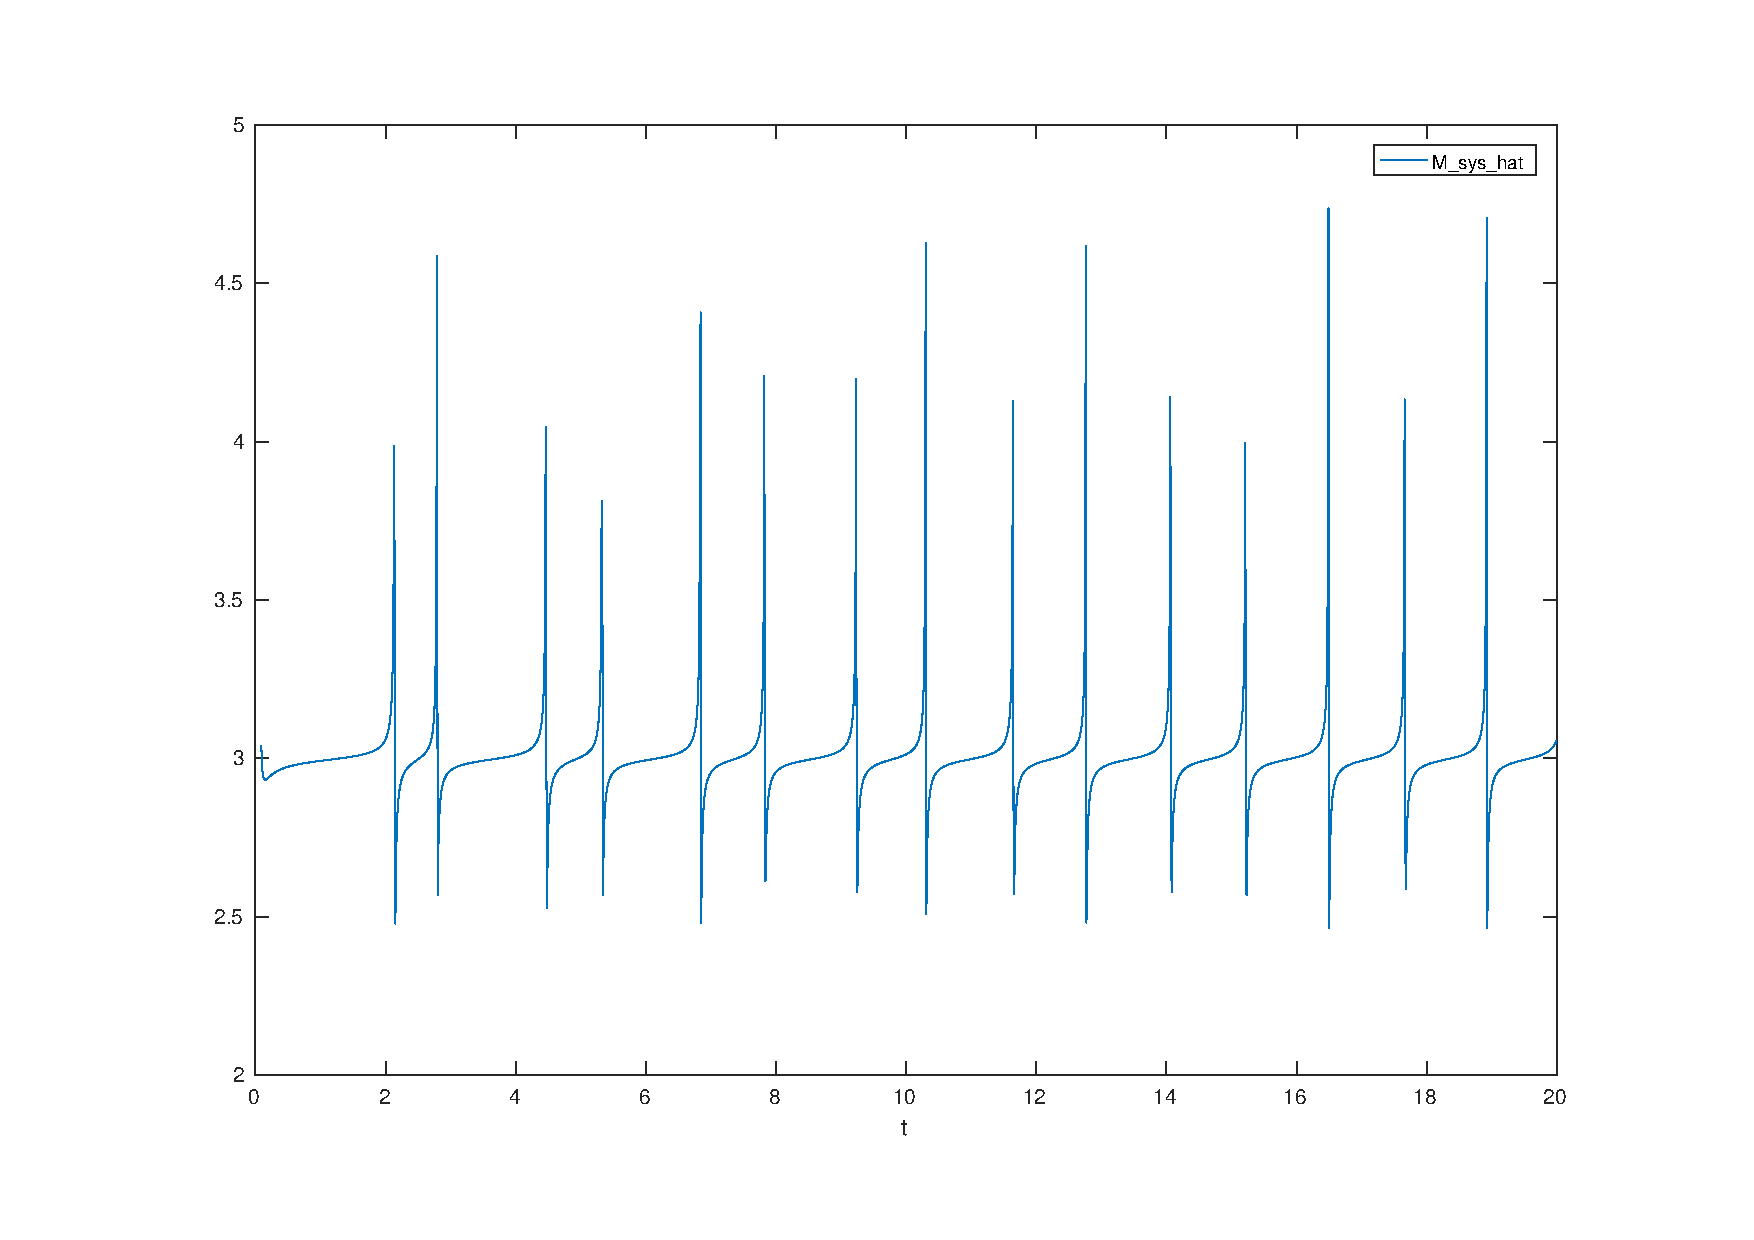
\includegraphics[width=0.99\linewidth]{system4_mass}
	\centering
	\caption{Estymacja masy układu z parametrami $T=0.01$, $k = 20$, $b = 1$, $m = 3$ dla 4 próbek optymalizacji. }
	\label{fig:system4_mass}
\end{figure}

\begin{figure}[H]
	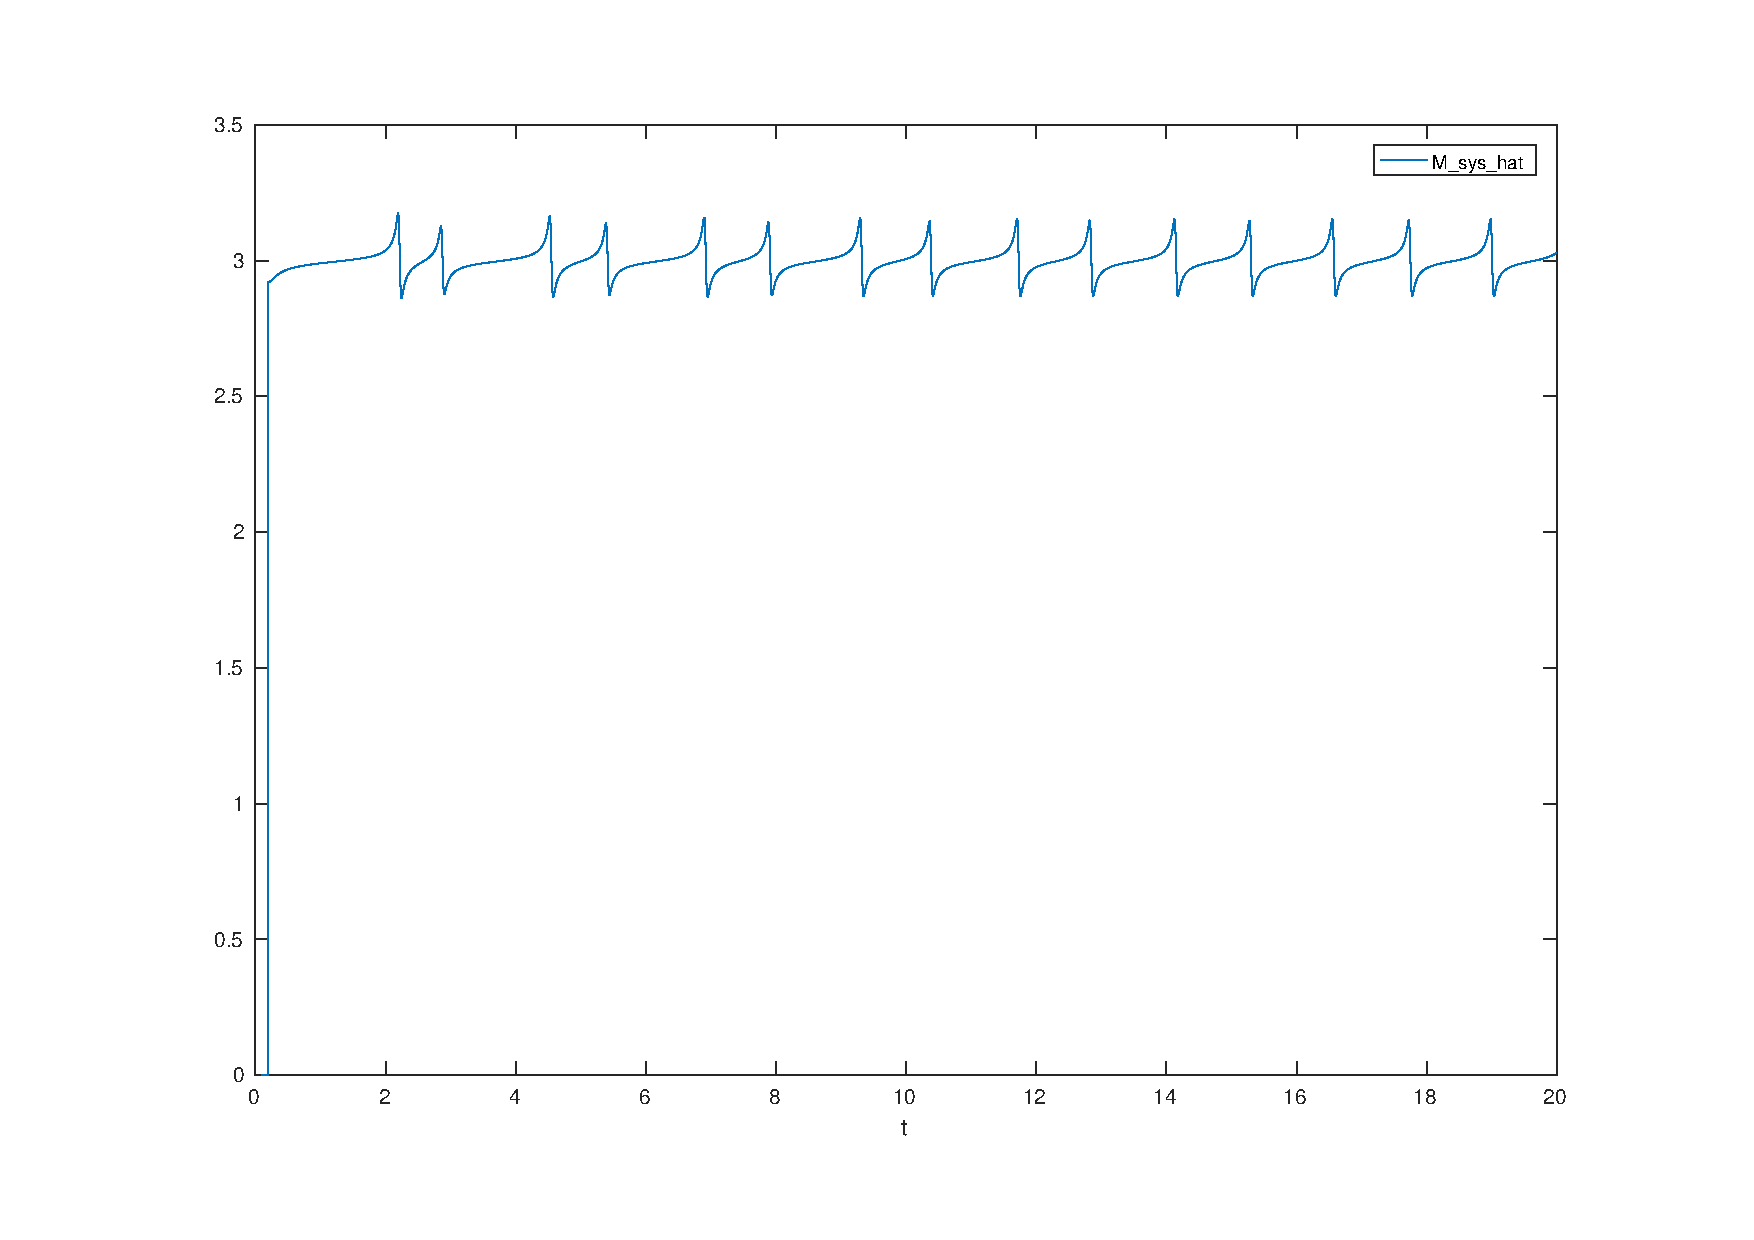
\includegraphics[width=0.99\linewidth]{system20_mass}
	\centering
	\caption{Estymacja masy układu z parametrami $T=0.01$, $k = 20$, $b = 1$, $m = 3$ dla 20 próbek optymalizacji.}
	\label{fig:system20_mass}
\end{figure}

\begin{figure}[H]
	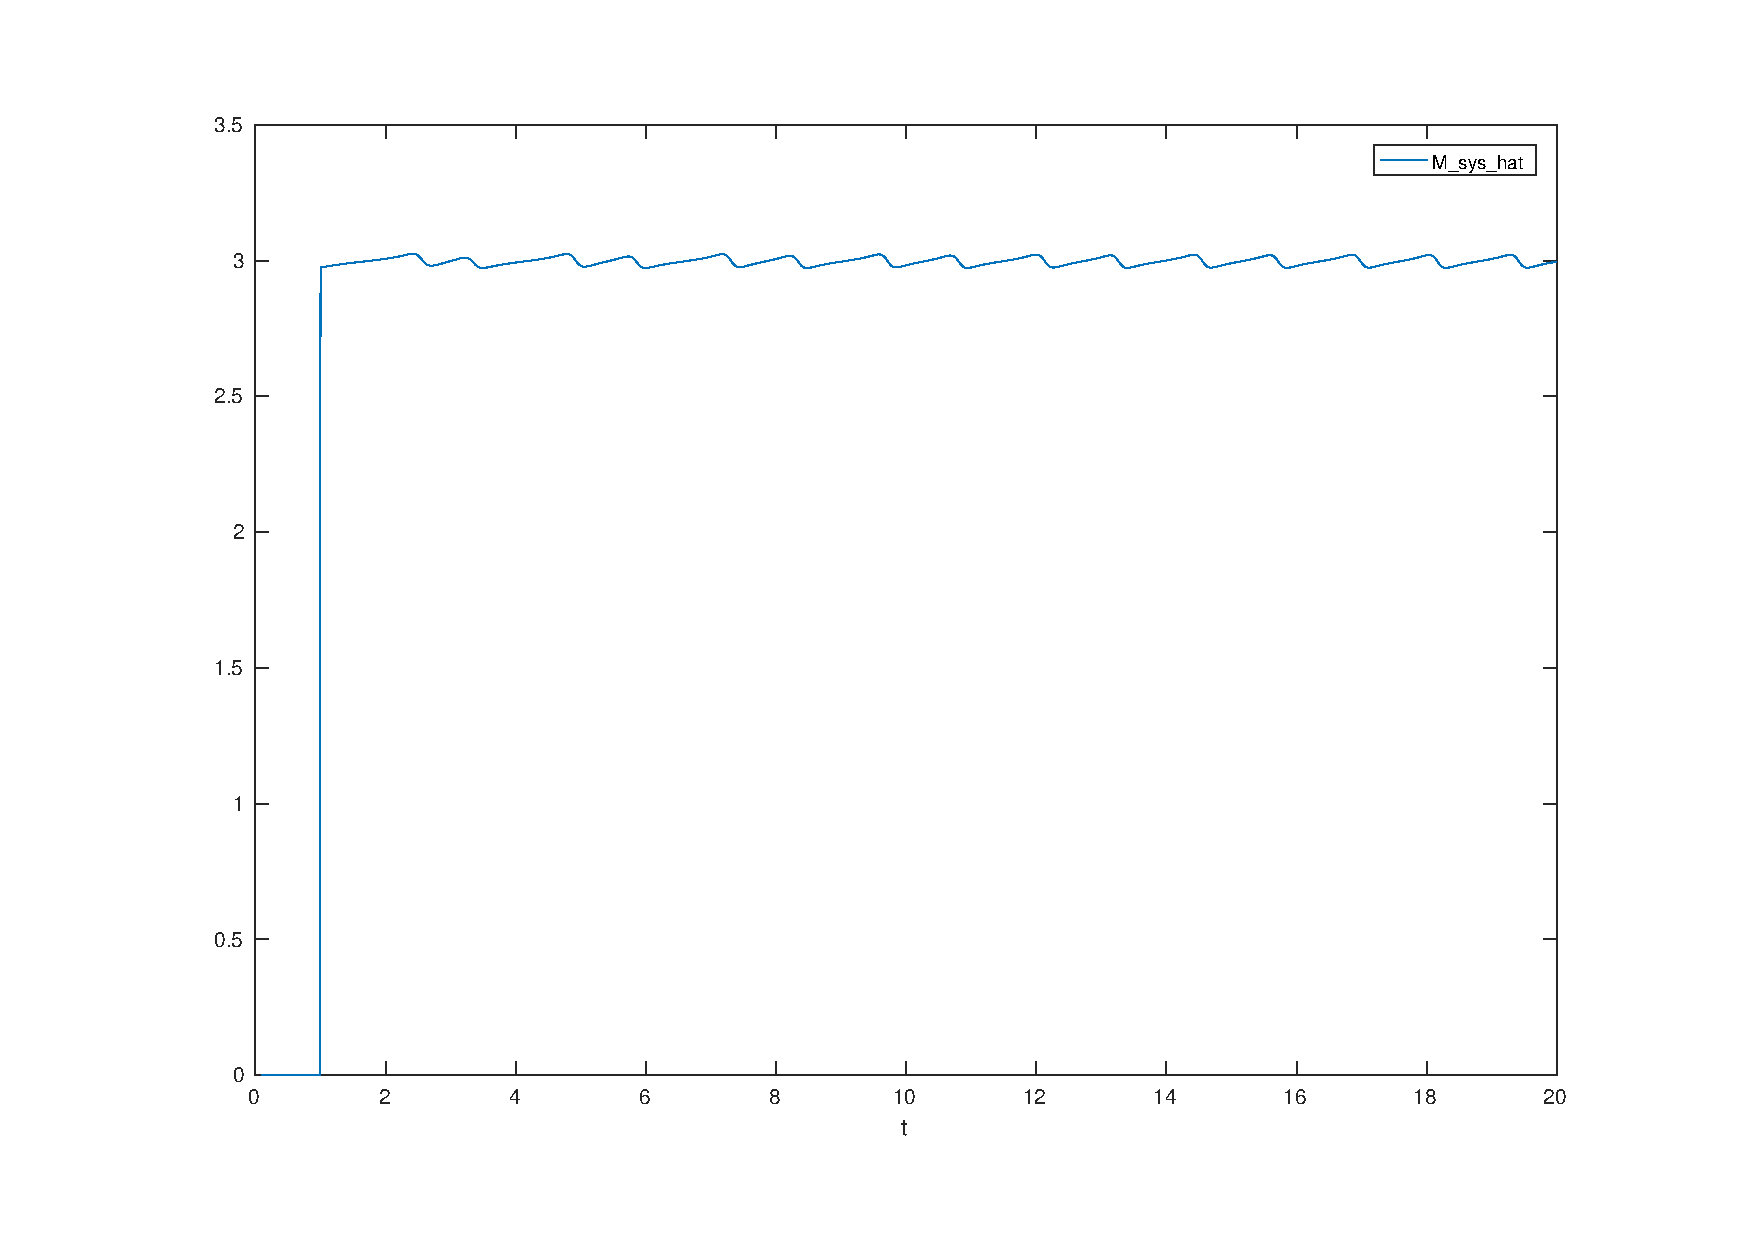
\includegraphics[width=0.99\linewidth]{system100_mass}
	\centering
	\caption{Estymacja masy układu z parametrami $T=0.01$, $k = 20$, $b = 1$, $m = 3$ dla 100 próbek optymalizacji.}
	\label{fig:system100_mass}
\end{figure}

\begin{figure}[H]
	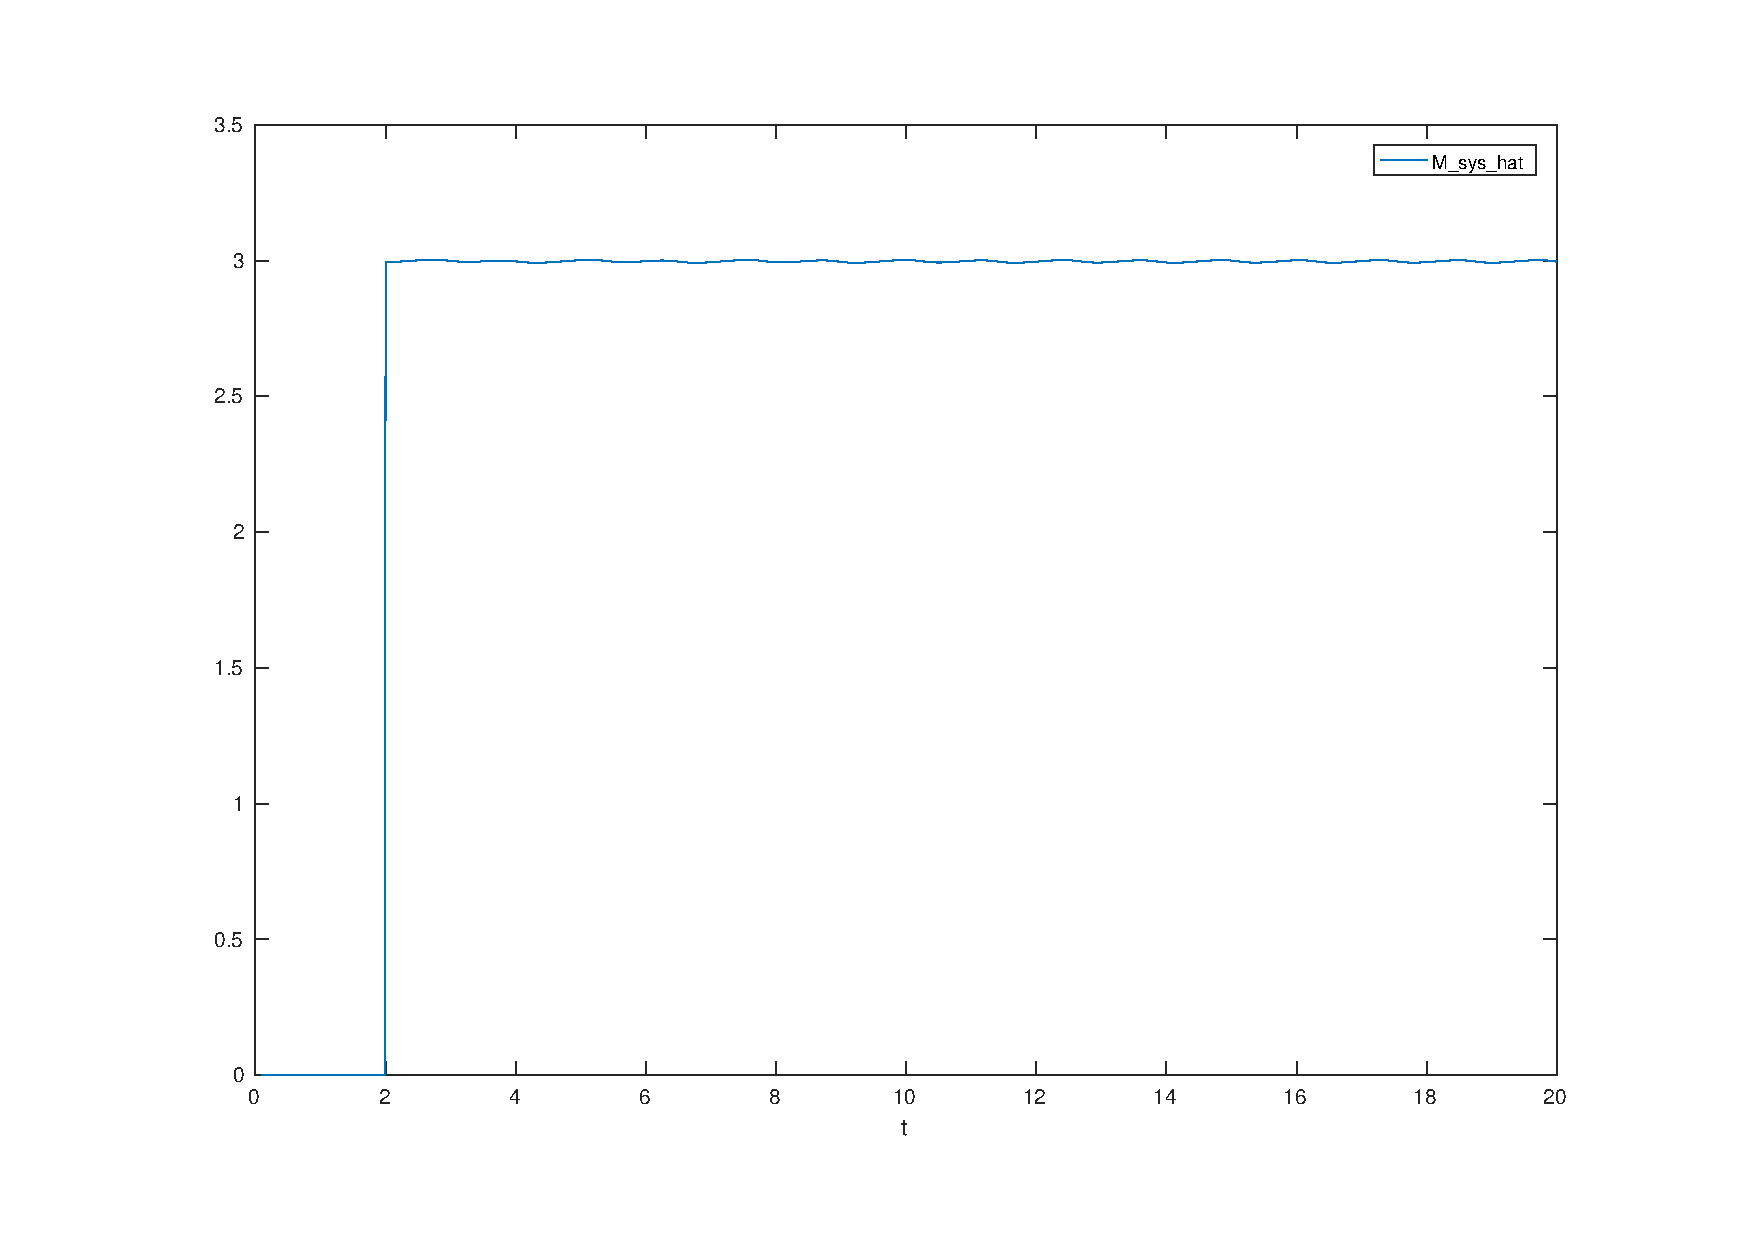
\includegraphics[width=0.99\linewidth]{system200_mass}
	\centering
	\caption{Estymacja masy układu z parametrami $T=0.01$, $k = 20$, $b = 1$, $m = 3$ dla 200 próbek optymalizacji.}
	\label{fig:system200_mass}
\end{figure}

\begin{figure}[H]
	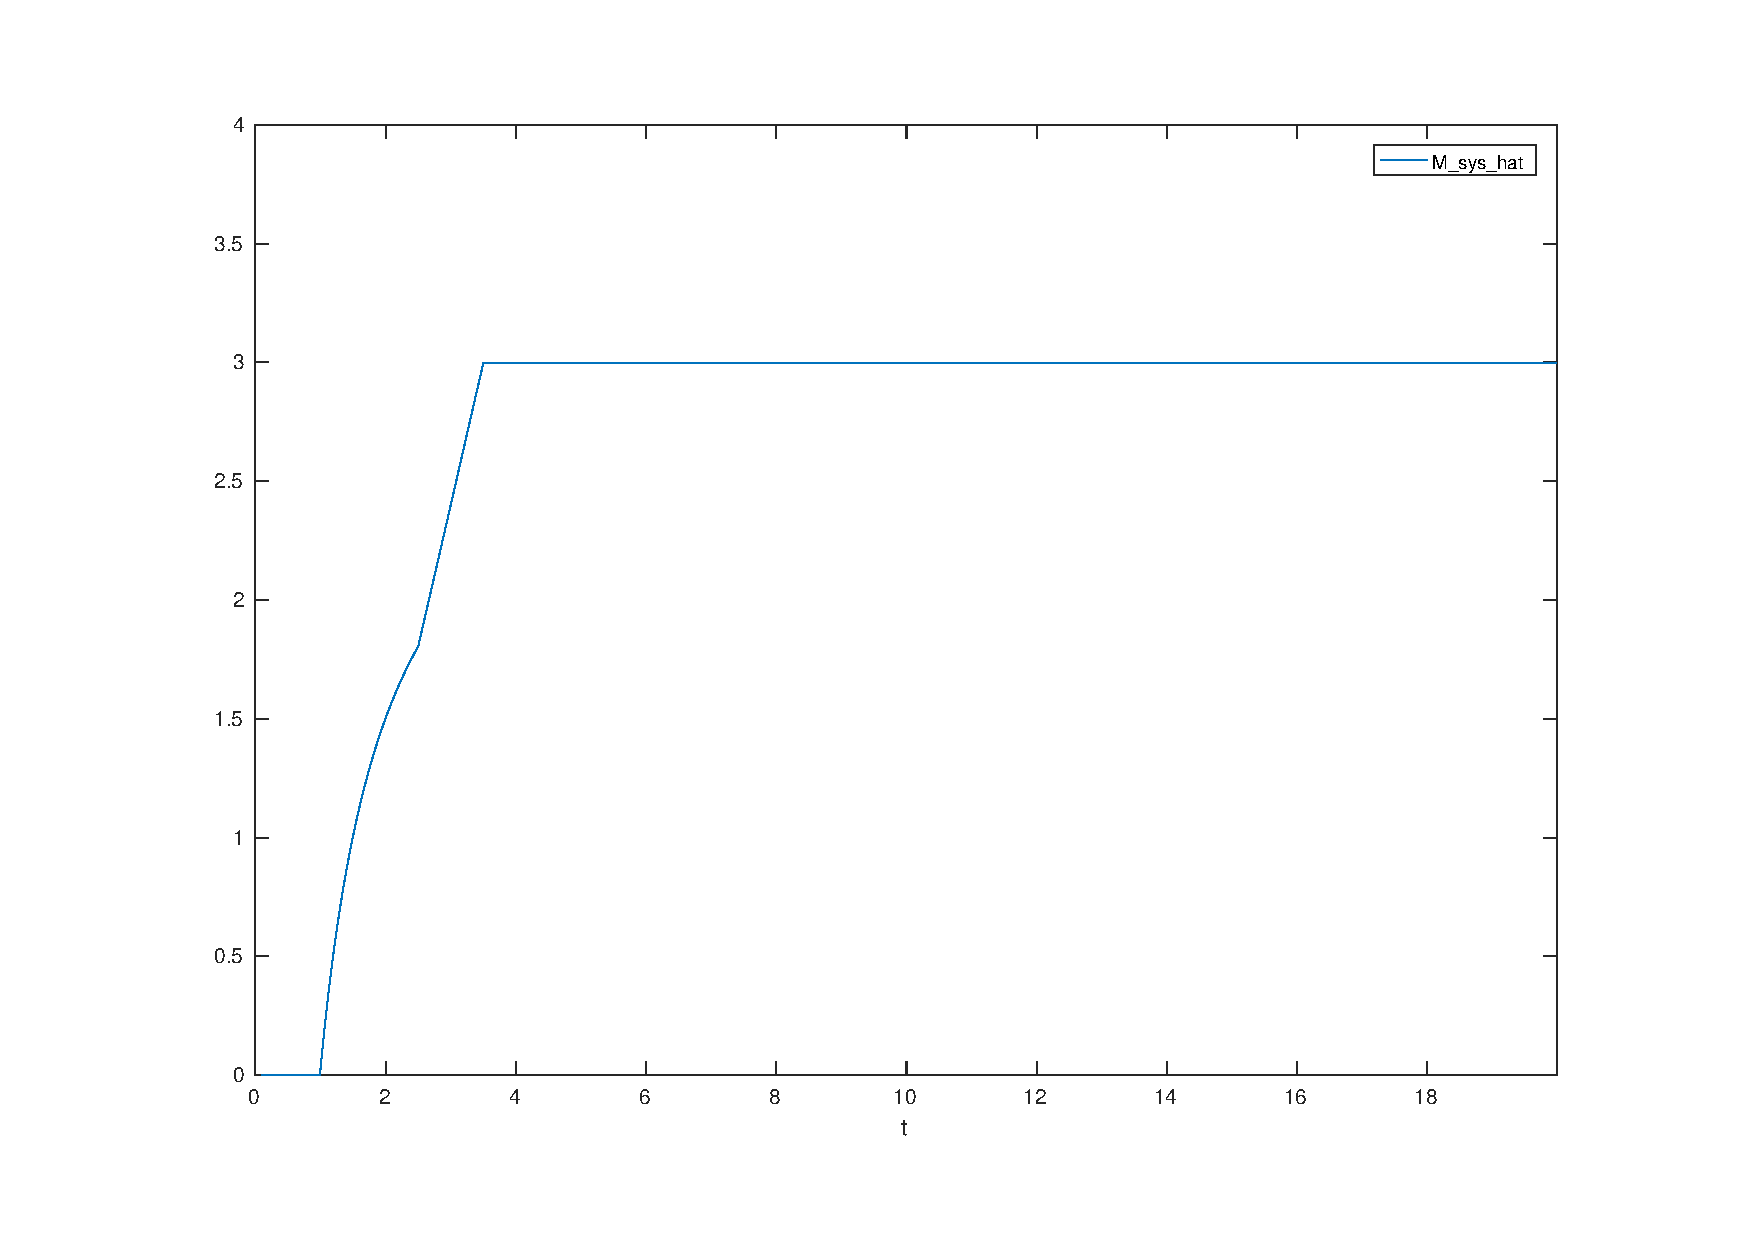
\includegraphics[width=0.99\linewidth]{filter_mass}
	\centering
	\caption{Estymacja masy układu z parametrami $T=0.01$, $k = 20$, $b = 1$, $m = 3$ dla 100 próbek optymalizacji i po zastosowaniu filtru średniej kroczącej.}
	\label{fig:filter_mass}
\end{figure}


\section{Kompensacja grawitacji}
Kompensacja polega na dodaniu do układu siły która przeciwdziała sile grawitacji masy.
W celu weryfikacji kompensacji siły grawitacji należy zastanowić się jak wyglądać powinny przebiegi układu. Można przyjąć, że układ powinien się zachowywać tak jakby nie była na nim zawieszona żadna masa (rys. \ref{fig:systemwm})
W idealnym przypadku (rys. \ref{fig:system_ideal}) układ zachowuje się jak ten pozbawiony masy. W normalnym przypadku (rys. \ref{fig:system_komp}), pomijając niedokładności, układ ze skompensowaną siłą grawitacji  zachowuje się dość dobrze Niwelowany jest wpływ grawitacji a układ stabilizuje się w porządanej pozycji. Kompensacja załączana jest stopniowo i nie uwzględnia energii układu która powstała przed załączeniem kompensacji. Powoduje to oscylacje widoczne w układzie. O tym jak szybko układ z załączoną kompensacją grawitacji się ustabilizuje decydują wartości zmiennych stanu układu w momencie rozpoczęcia kompensacji.


\begin{figure}[H]
	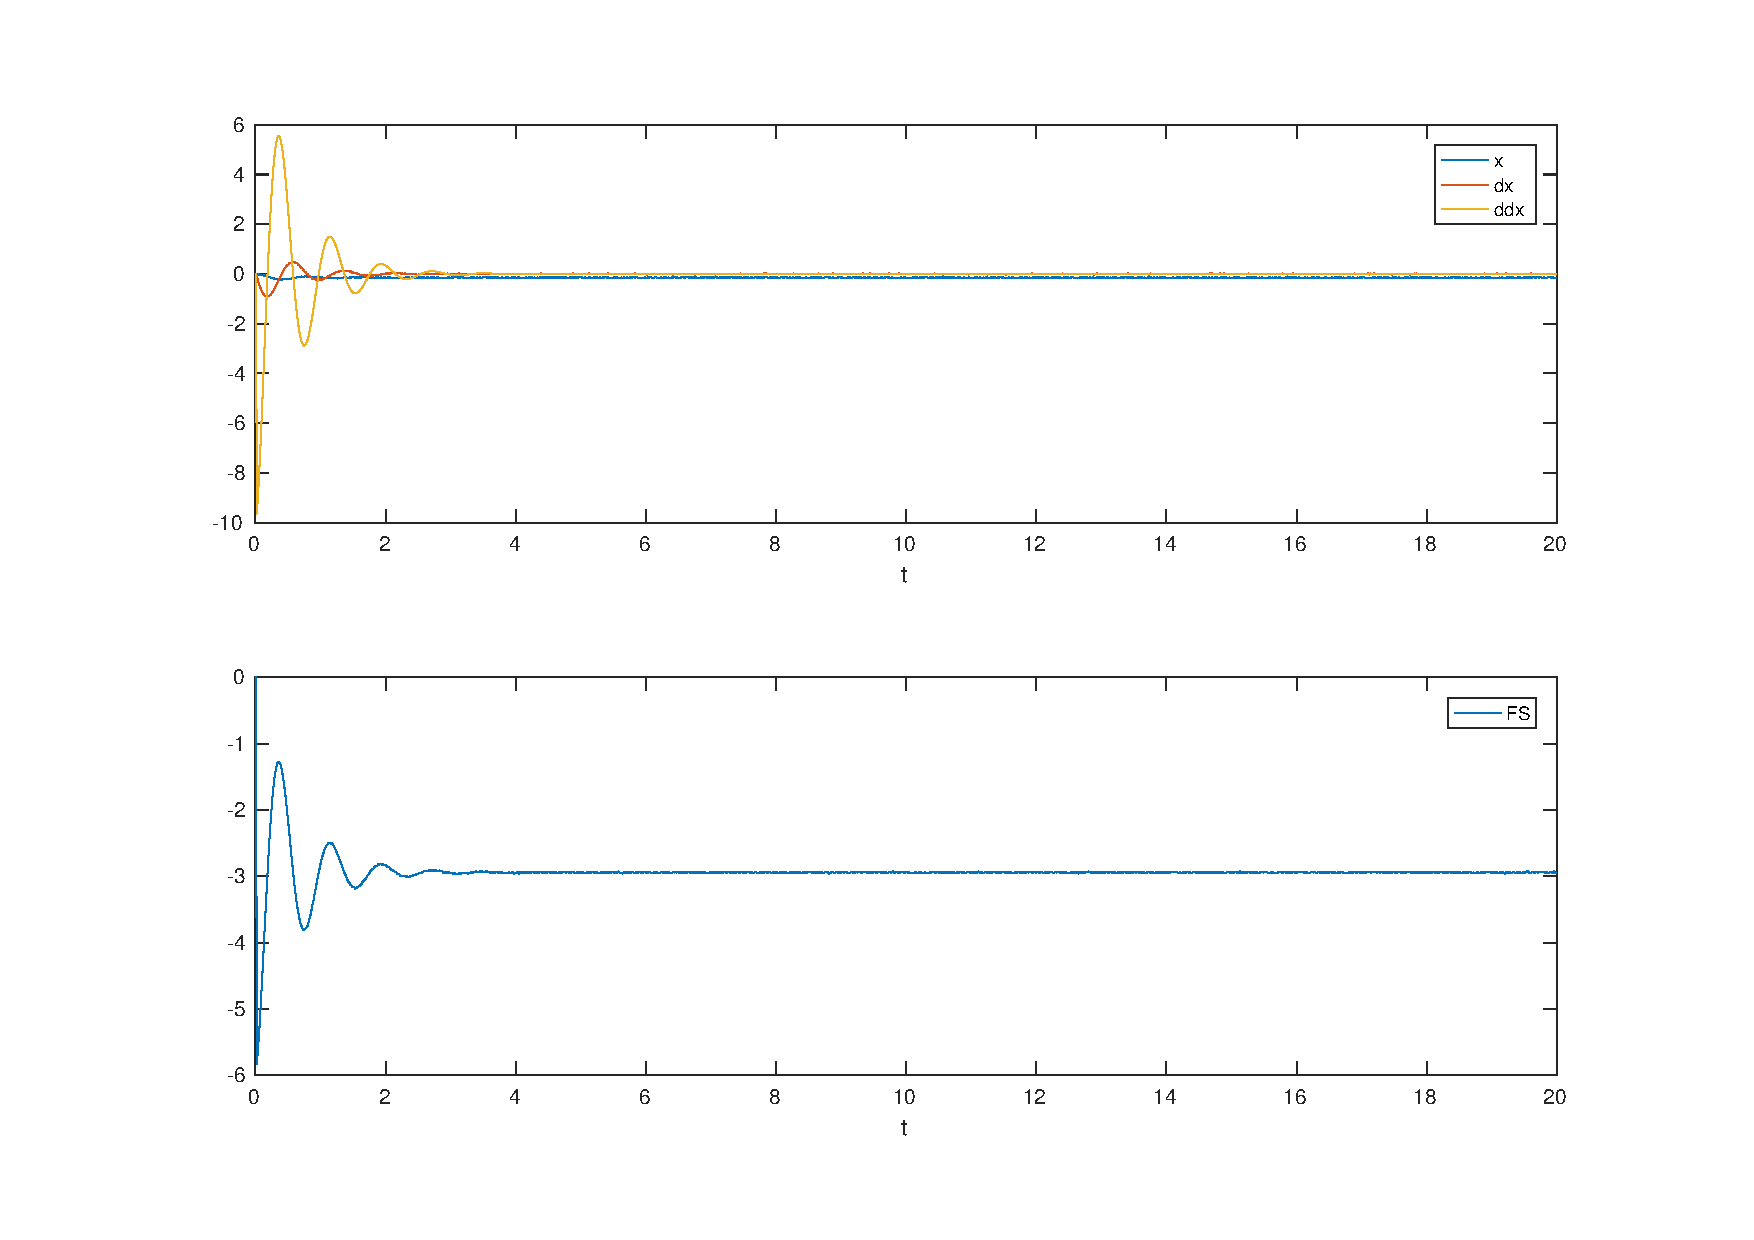
\includegraphics[width=0.99\linewidth]{system_wm_sys}
	\centering
	\caption{Symulacja układu z parametrami $T=0.01$, $k = 20$, $b = 1$, $m = 0.3$. Masa jest 10 razy mniejsza niż początkowego układu.}
	\label{fig:systemwm}
\end{figure}

\begin{figure}[H]
	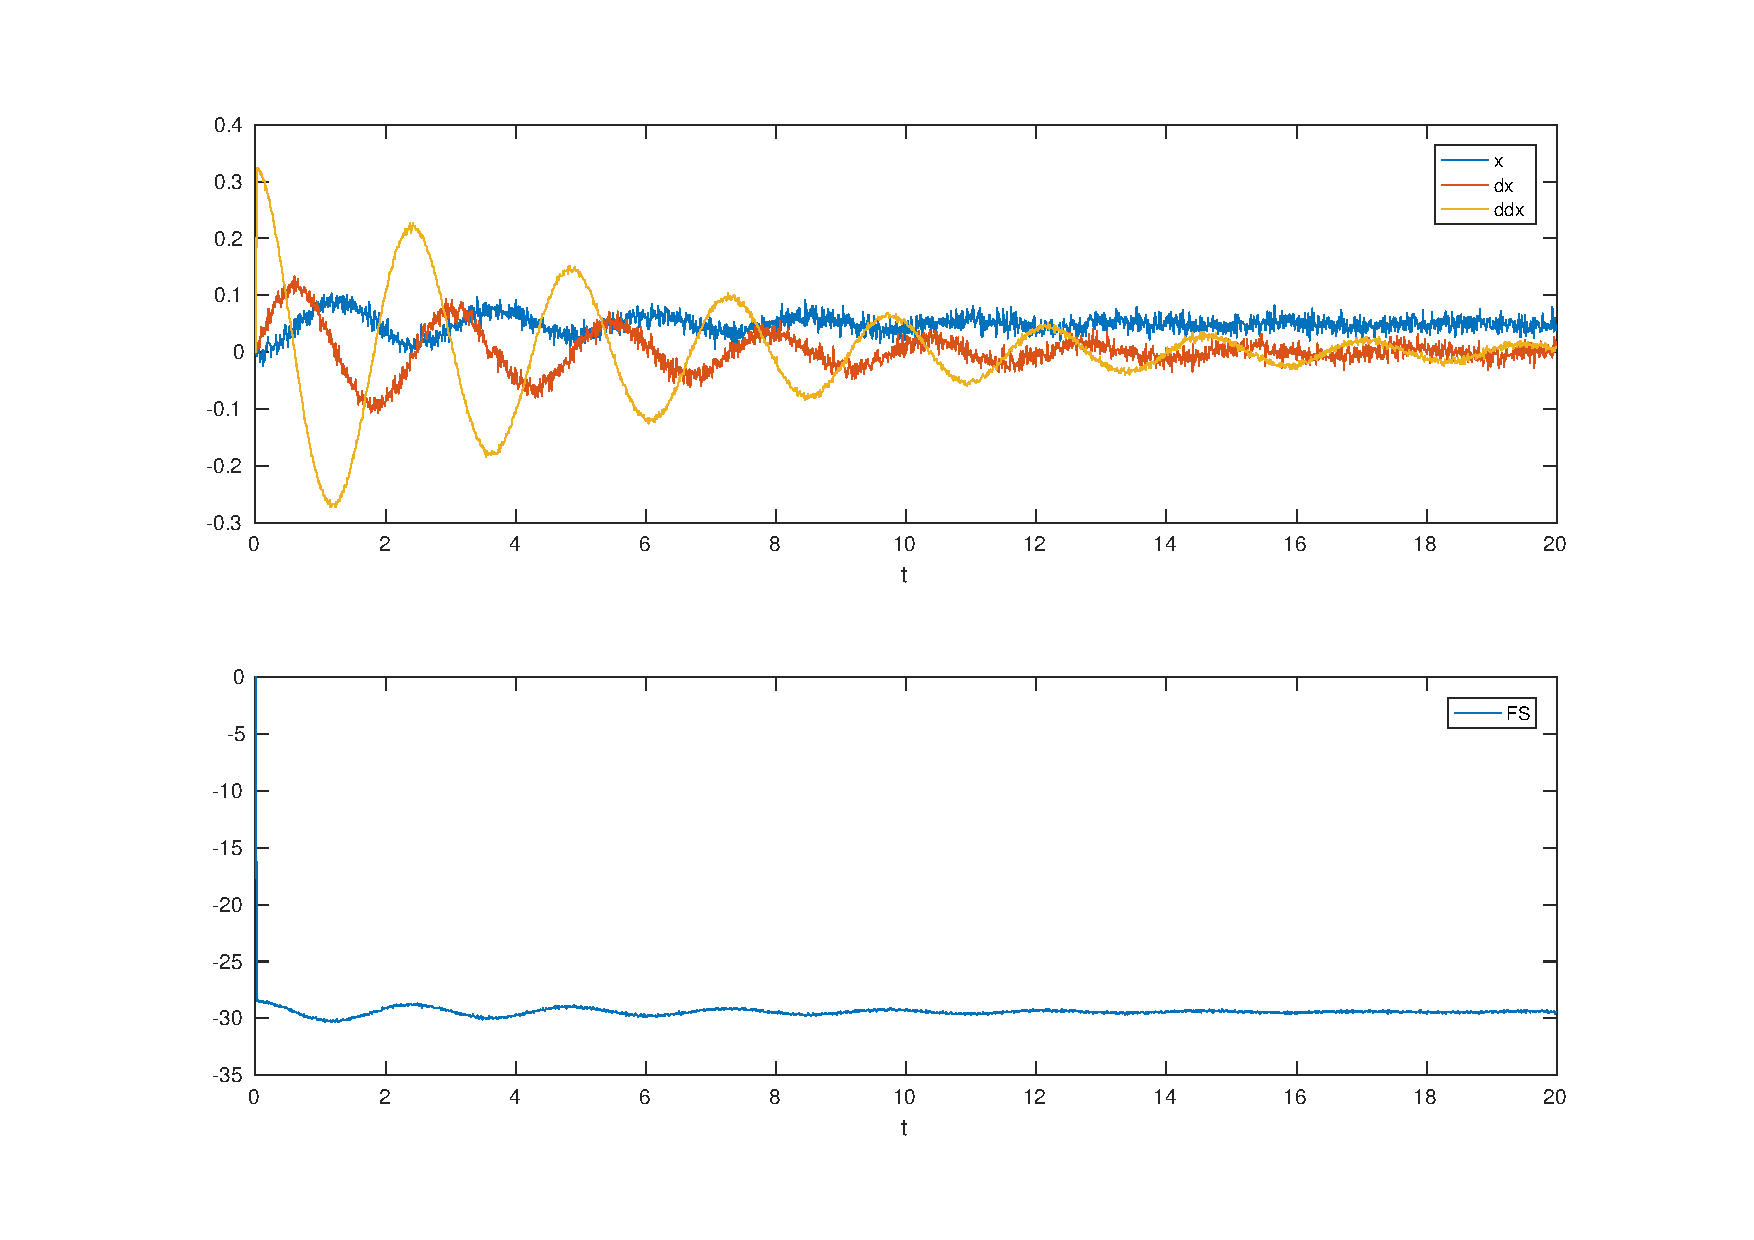
\includegraphics[width=0.99\linewidth]{grav_ideal_sys}
	\centering
	\caption{Symulacja układu z parametrami $T=0.01$, $k = 20$, $b = 1$, $m = 0.3$. Oraz załączoną kompensacją grawitacji.}
	\label{fig:system_ideal}
\end{figure}

\begin{figure}[H]
	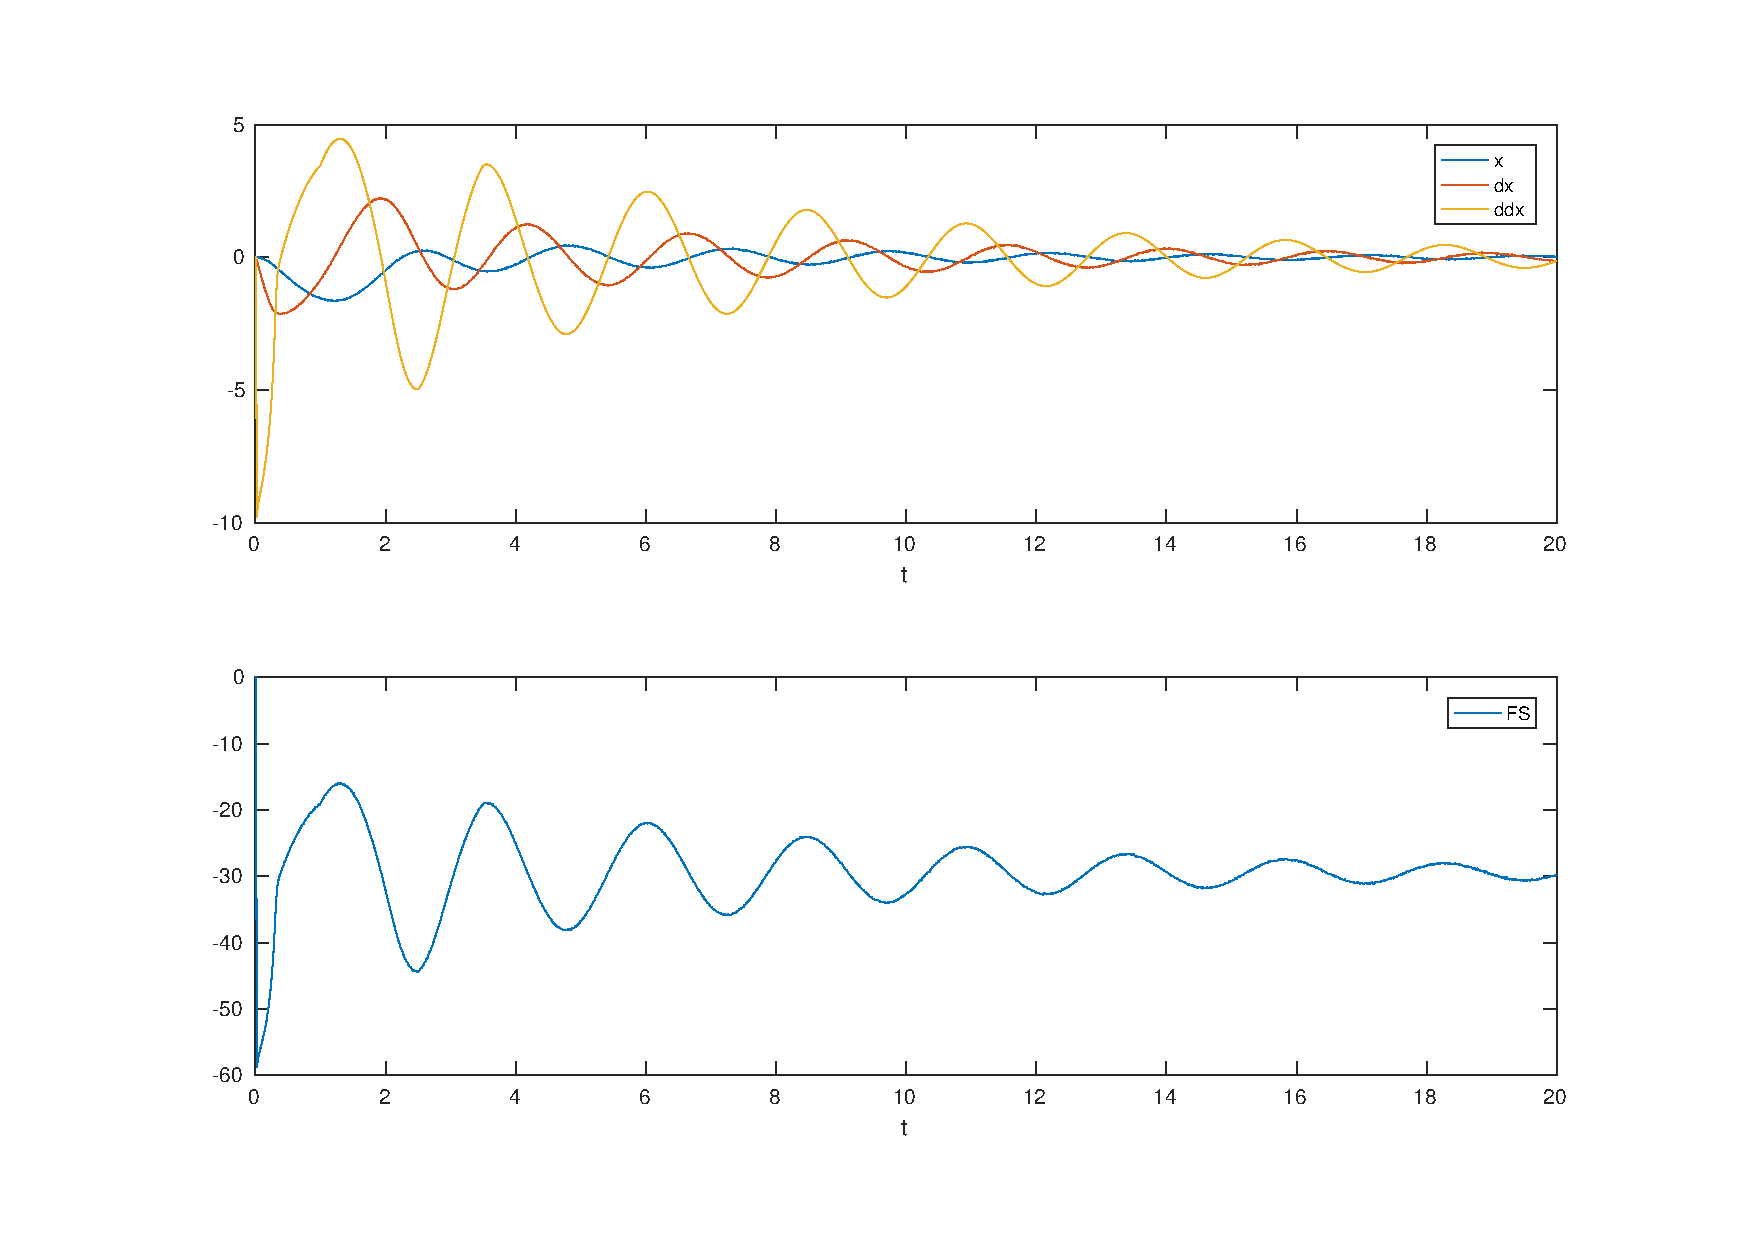
\includegraphics[width=0.99\linewidth]{grav_normal_sys}
	\centering
	\caption{Symulacja układu z parametrami $T=0.01$, $k = 20$, $b = 1$, $m = 0.3$. Oraz załączoną kompensacją grawitacji.}
	\label{fig:system_komp}
\end{figure}

\end{document}